\documentclass{UoYCSproject}{}
\title{Undecided Title}
\author{Callum Hewitt}
\supervisor{Lilian Blot}
\date{2016 Oct 12}
\wordcount{2}
\BSc
\abstract{
Not completed
}
\dedication{Not completed}
\acknowledgements{
	Not completed
}

\usepackage{listings}
\usepackage{graphicx}
\usepackage{xcolor}
\usepackage{usebib}
\usepackage{tikz}
\usepackage{amsmath}
\usepackage{amssymb}
\usepackage{color,soul}

\bibinput{bibliography}
\newcommand\todo[1]{\emph{{\textcolor{red}{TODO: #1}}}}
\newcommand\newtext[1]{\emph{{\textcolor{blue}{#1}}}}
\newcommand\revisit[1]{\hl{#1}}
\newcommand\citetitle[1]{\usebibentry{#1}{title}}

\graphicspath{{images/}}

\usetikzlibrary{shapes,arrows,positioning}
\tikzset{
  font={\fontsize{6pt}{6}\selectfont}
  }
\tikzstyle{startstop} = [rectangle, rounded corners, text centered, draw=black, fill=red!15,text width=2cm]
\tikzstyle{io} = [trapezium, trapezium left angle=70, trapezium right angle=110, text centered, draw=black, fill=blue!15,text width=2cm]
\tikzstyle{process} = [rectangle, text centered, draw=black, fill=orange!15,text width=3cm]
\tikzstyle{decision} = [diamond, aspect=2, text centered, draw=black, fill=green!15,text width=2cm]
\tikzstyle{bigdecision} = [regular polygon, regular polygon sides=6, xscale=3, text centered, draw=black, fill=green!15, text width=5cm]
\tikzstyle{arrow} = [thick,->,>=stealth]

\begin{document}
\maketitle
\listoffigures
\listoftables

\chapter{Introduction}
\label{cha:Introduction}

The terms 'autonomous vehicle' and 'self-driving car' were once thought of as science fiction, but as of recent, they have become our reality. Google's Self-Driving Car Project is gaining traction, with cars currently driving \newtext{in Milton Keynes and }four different US states \citep{GoogleCars}. Tesla Motors have deployed a beta version of their Autopilot system into all of their vehicles produced since September 2014. The system has been blamed for both saving and ending lives \citep{TeslaHospital} \citep{TeslaUnderInvestigation}. 2016 has been a big year for autonomous vehicles and with that comes an even bigger push for robust and secure autonomous systems.
The possible benefits of autonomous vehicles cover a lot of different areas of concern. 

The main issue it addresses is safety. Autonomous vehicles would be able to react to incidents on the road much more quickly than a human driver would. A human's 'thinking distance' can often determine whether someone survives an accident or not. This distance can also be greatly increased if the driver of the vehicles is under the influence of alcohol or narcotics. An autonomous vehicle however, would be able to react to accidents much more quickly than a human, reducing the thinking distance greatly, improving road safety.

\begin{figure}[h]
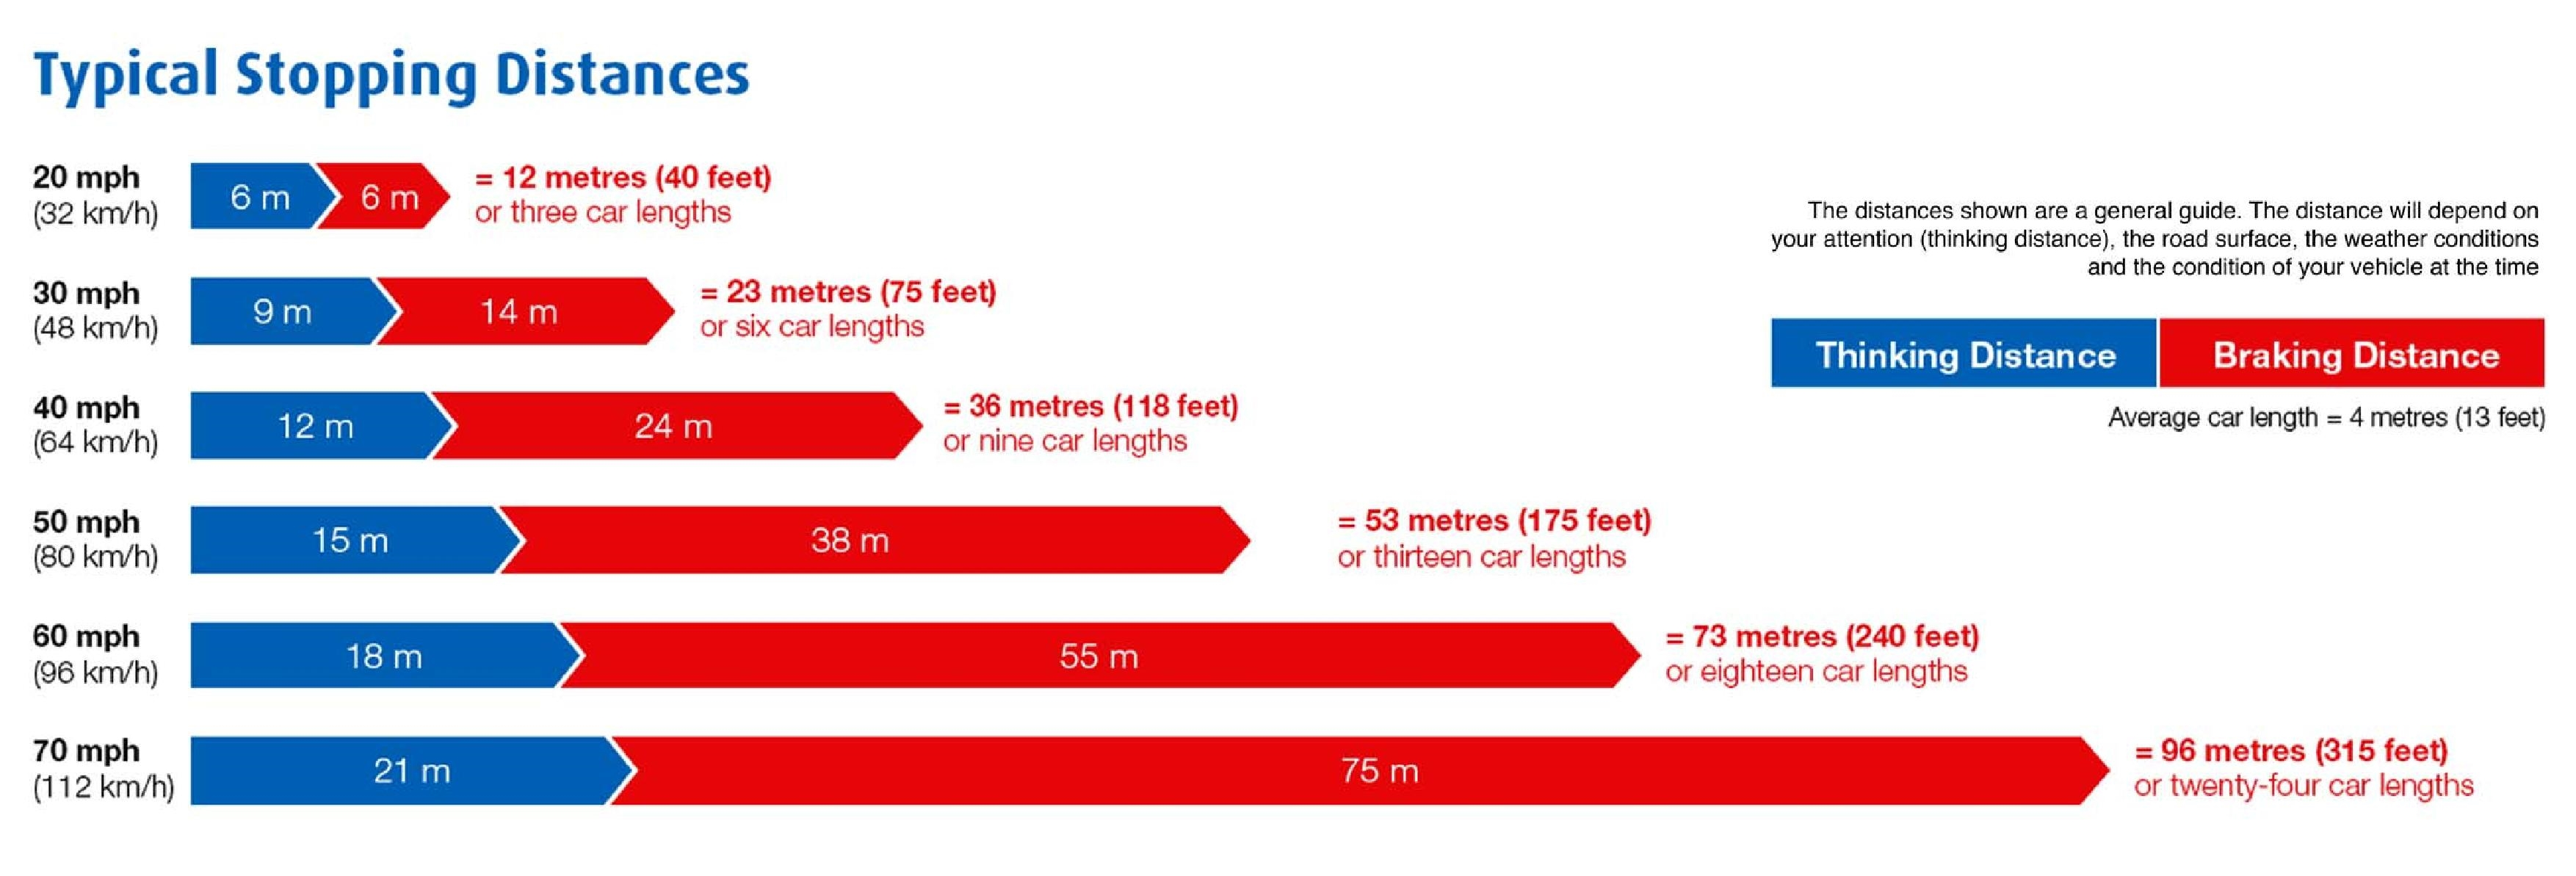
\includegraphics[width=\textwidth]{stoppingDistances.jpg}
\caption{Diagram from Rule 126 in the UK Highway Code \citep{StoppingDistances}}
\end{figure}

Autonomous vehicles could also make transport more efficient. Research by Mersky in April 2016 suggested that fuel conservation control strategies could make autonomous vehicles up to 10\% more fuel efficient than current EPA fuel economy test results \citep{Mersky2016} \todo{Read this article}. Having vehicles which are fuel efficient is becoming increasingly important, with landmark climate change deals such as 'The Paris Agreement' introducing limits on greenhouse gas emissions globally. The introduction of electric vehicles into the car market is also an important factor to consider, as the range of such vehicles still has not managed to match that of their gasoline counterparts. More efficient driving strategies introduced by autonomous vehicles could reduce this gap.

\newtext{Congestion contributes to fuel loss in quite a large way. In the US in 2014 an estimated 3.1 billion gallons (11.7 billion litres) of fuel was wasted due to congestion \citep{Schrank2015}. Automating typical driving activities and communications between vehicles, in situations such as lane changes, could reduce congestion and improve efficiency. Unsafe lane changes don't even have to result in a crash to cause delays. If a car brakes due to a car merging unsafely it can cause a ripple effect, creating a traffic jam.}

Autonomous vehicles also offer a level of comfort not currently available today. In a world where autonomous vehicles are commonplace, it is not hard to imagine people doing work, reading or relaxing in their car instead of having to focus on driving. 

However, today there are still a number of concerns surrounding autonomous vehicles. One of the major concerns is over the reliability of the systems governing the vehicle. These systems need to be responsive and accurate and they cannot afford to fail in such safety critical environments. Already concerns over Tesla's Autopilot system are impacting the image of the company, and the system isn't even out of beta testing yet \citep{TeslaCriticised}. 

In order to address these concerns safely, we can create simulations which test our autonomous systems. These simulations can test the reliability of our systems. Researchers at the University of Texas set up the Autonomous Intersection Management (AIM) project, which aims to " create a scalable, safe, and efficient multiagent framework for managing autonomous vehicles at intersections" \citep{AIMProject}. The project managed to apply their tested intersection software in a mixed reality test using a real life autonomous vehicle \citep{Quinlan2010}, demonstrating how simulations are vital tools when testing these safety critical systems.

\newtext{In this project we make a number of assumptions. Firstly we assume that the sensors resolving the positions of the vehicle and it's surrounding obstacles are perfectly accurate. We also assume that the vehicle can communicate reliably with other vehicles. These assumptions are existing areas of research for autonomous vehicles but are not considered in this paper. The main focus here is on how autonomous vehicles can self-organise to minimise delays in traffic with effective, safe lane merging.}

The aims of this project are as follows:
\begin{itemize}
\item Attempt to generalise the AIM codebase such that other simulations can be created for non-intersection related situations.
\begin{itemize}
\item If the codebase proves difficult to refactor, new simulator code will need to be created
\end{itemize}
\item Use the new codebase to create a decentralised system for managing lane merging.
\item Use the new codebase to create a centralised system for managing lane merging.
\item Compare the effectiveness of both strategies.
\end{itemize}

Creating these simulations helps to determine the effectiveness of two different strategies and also provides a codebase within which future simulations for other situations can be created.
\chapter{Literature Review}
\label{cha:Literature Review}

\section{Car Following Models}
\label{sec:Car Following Models}
Most lane changing models stem from 'car-following models', which define actions for a vehicle based on the behaviour of its predecessors (the vehicles in front of it). One early car-following model was defined in 1981 by P.G. Gipps \citep{Gipps1981}. It was designed to mimic real-world driver behaviour, calculating a safe travel speed for a vehicle based on the speed of its predecessor. A safe travel speed is defined as a speed at which the driver can safely stop if the preceding driver stops.

Gipps' paper defines two equations, which provide constraints on the speed of vehicle $n$ at time $t + \tau$. $t$ is the current time and $\tau$ is the apparent reaction time, a constant for all vehicles. The first equation defines the acceleration constraint of the vehicle. It was obtained using measurements from an instrumented car.

\begin{equation}\label{Gipps1981Accel}
v_n(t+\tau) \leqslant v_n(t) + 2.5a_n\tau\Biggl(\frac{1 - v_n(t)}{V_n}\Biggr)\Biggl(\frac{0.025 + v_n(t)}{V_n}\Biggr)^{1/2}
\end{equation}

$v_n(t)$ is the speed of vehicle $n$ at time $t$. $a_n$ is the maximum acceleration the driver of vehicle $n$ wishes to undertake. $V_n$ is the target speed for vehicle $n$. The equation shows that the driver accelerates until close to their target speed. They then reduce their acceleration until it reaches zero. At this point the vehicle should be travelling at it's target speed.

The second constraint is the braking profile of the vehicle. This is given as

\begin{equation}\label{Gipps1981Brake}
\begin{split}
&v_n(t+\tau) \leqslant \\
&b_n\tau + \sqrt{\Biggl(b_n^2\tau^2 - b_n\biggl(2\Bigl[x_{n-1}(t) - s_{n-1} - x_n(t)\Bigr] - v_n(t)\tau - \frac{v_{n-1}(t)^2}{\hat{b}}\biggr)\Biggr)}
\end{split}
\end{equation}

$b_n$ is the most severe braking the driver of vehicle $n$ wishes to undertake. It is always a negative value, and should be considered negative acceleration. $\hat{b}$ is the driver of vehicle $n$'s best guess at $b_{n-1}$ where $n-1$ is $n$'s predecessor. $x_n(t)$ is the location of the front of vehicle $n$ at time $t$. $s_n$ is the effective size of vehicle $n$. This is equal to the physical length of $n$, plus a margin $n$'s successor is not willing to enter, even when $n$ is at rest.

Therefore, at time $t + \tau$, assuming the driver travels as fast as is safe, and within the limitations of the vehicle, the speed is given by the minimum of these two equations.

\begin{equation}
v_n(t) = \min{(\eqref{Gipps1981Accel},\eqref{Gipps1981Brake})}
\end{equation}

This model works well at describing the behaviour of traffic. However, translating this work to autonomous vehicles poses a number of problems. Firstly, the work is based on the behaviour of real-world drivers in instrumented vehicles. This introduces human driver variables into the equations. An autonomous vehicle with perfect sensors would have an almost negligible $\tau$, as the vehicles would have a very minimal reaction time. $s_n$ would also need to be adjusted. The margin added can be much less, as autonomous vehicles would be more precise than human drivers, driving closer to their predecessors. 

The model also ignores inter-vehicle communication. Autonomous vehicles could communicate their intentions to nearby vehicles, allowing them to act before they do. This could greatly reduce the following distance of successor vehicles, it would also allow vehicles to accelerate and move as a unit, or a 'platoon'. It would also allow autonomous vehicles to gain accurate value for $\hat{b}$.

In 2000 Treiber et al. suggested the 'Intelligent Driver Model' (IDM). In the IDM, the acceleration of vehicle $\alpha$, $\dot{v_\alpha}$, is defined using a continuous function of its velocity, $v_\alpha$; the distance to the rear of its predecessor, $s_\alpha$; and the velocity difference of $\alpha$ and it's predecessor, also known as the approaching rate $\Delta v_\alpha$. The vehicle interactions are solely based on $\alpha$'s relative acceleration to its predecessor. The model only provides position information for a vehicle in relation to its predecessor, and it does not provide its velocity at a given time, as Gipps' model does. 

The IDM is broken into two components. The first describes the behaviour of a vehicle on a free road.

\begin{equation}
\dot{v_\alpha} = a^{(\alpha)}\Biggl[1 - \biggl(\frac{v_\alpha}{v_0^{(\alpha)}}\biggr)^\delta\Biggr]
\end{equation}

Here $a^{(\alpha)}$ is the maximum acceleration of vehicle $\alpha$ and $v_0^{\alpha}$ is the desired velocity of $\alpha$. $\delta$ is the acceleration exponent, which is typically 4. 

The second component describes the behaviour of a vehicle as it approaches its predecessor. 

\begin{equation}
\dot{v_\alpha} = - a^{(\alpha)}\biggl(\frac{s^*}{s_\alpha}\biggr)^2
\end{equation}

As the gap, $s_\alpha$, between $\alpha$ and it's predecessor, gets closer to the desired minimum gap $s^*$, $\alpha$ decelerates.

Interpolating the two components gives us the IDM. 

\begin{equation}
\dot{v_\alpha} = a^{\alpha}\Biggl[1 - \biggl(\frac{v_\alpha}{v_0^\alpha}\biggr)^\delta - \biggl(\frac{s^*(v_\alpha,\Delta v_\alpha)}{s_\alpha}\biggr)^2\Biggr]
\end{equation}

The desired minimum gap in the IDM varies dynamically with velocity and approaching rate. It is given by the following function.

\begin{equation}\label{IDMSpacingFunction}
s^*(v,\Delta v) = s_0^{(\alpha)} + s_1^{(\alpha)}\sqrt{\frac{v}{v_0^{(\alpha)}}} + T^\alpha v + \frac{v\Delta v}{2\sqrt{a^{(\alpha)}b^{(\alpha)}}}
\end{equation}

The equation takes the bumper-to-bumper space $s_0^{(\alpha)}$, also known as the minimum jam distance, and adds the comfortable jam distance $s_1^{(\alpha)}$. The bumper-to-bumper space is the minimum gap between $\alpha$ and its predecessor in stationary traffic. The comfortable jam distance is an extra distance added on for comfort, and to allow for a slower driver reaction time. In the paper, this value is set to $0$. We can also consider it negligible for autonomous vehicles. $T$ is the safe time headway; it represents the time required for the vehicle to safely come to a stop. Finally $b^{(\alpha)}$ is the desired deceleration for $\alpha$.

The IDM does not attempt to directly mimic human behaviour in traffic situations. It models a general acceleration and braking profile for a given vehicle. As such, it is well suited for adaptation by autonomous vehicle models, as seen in \citep{Kesting2007}. However, similarly to Gipps' model, the standard IDM only applies to single lane traffic. It also ignores inter-vehicle communication and platooning opportunities. 

In vehicle platoons, such as those analysed by Kamali in 2016 \citep{Kamali2016}, each vehicle autonomously follow it's predecessor, with the lead vehicle controlling the overall pace of the platoon. Platoons make heavy use of vehicle-to-vehicle (V2V) communication to allow vehicles to join and leave, as well as to continuously control vehicle spacing and velocity.

Kamali developed a model for an automated platoon, defining procedures for vehicles joining and leaving. 

A joining vehicle can integrate at either the back or the middle of the platoon. The vehicle first sends a join request to the platoon leader. If the vehicle is at the back of the platoon the leader sends an agreement and the vehicle follows its predecessor. If the vehicle requests to join in front of another platoon vehicle, the leader first asks the platoon vehicle to increase space; once the space is large enough for the joining vehicle, the leader sends an agreement. The joining vehicle then manoeuvres into the space and follows the preceding vehicle. Having now joined the platoon, the vehicle sends a confirmation to the leader. The leader then requests that the vehicle that gave way for the joining vehicle decreases their spacing back to normal.

A leaving vehicle sends a request to the leader. When it receives permission to leave the vehicle increases its spacing from its predecessor; once the vehicle is at its maximum distance from its predecessor the vehicle can change lanes. Once out of the convoy the vehicle sends an acknowledgement to the leader.

This model isn't very strict, acting as more of a set of requirements than a true model. The paper sets the requirements using pre-defined gaps, and has no strict calculations guiding following characteristics. It could be implemented using spacing rules from both the IDM and Gipps' model, however, by using V2V communication, the lead vehicle can control the actions of all vehicles in its platoon. Instead of using IDM or Gipps' model, the lead vehicle can control the gaps between vehicles so that they all increase and decrease simultaneously. The gaps could be based on the platoon's velocity, perhaps using \eqref{IDMSpacingFunction} from the IDM. By centralising control in this way, vehicle platoons can avoid the traffic shock effect \citep{Daganzo1994}.

\section{Centralised and Decentralised}
\label{sec:Centralised and Decentralised}

We can divide approaches to autonomous vehicles into centralised and decentralised solutions. Centralised solutions rely on an external agent to manage vehicles. Vehicles use vehicle-to-infrastructure (V2I) communication channels to send information and receive instructions from the external agent. Decentralised solutions use vehicle-to-vehicle (V2V) communication to let other vehicles know their state, their intentions and to arrange any complex actions that might affect surrounding vehicles.

\subsection{Centralised Systems}
\label{subsec:Centralised Systems}
The Autonomous Vehicle Intersection management system (AIM) described in \citep{Dresner2004} is an example of a centralised V2I system. The system works by dividing the intersection into a grid of $n \times n$ reservation tiles. Drivers 'call ahead' to the intersection sending information packets containing

\begin{enumerate}
\item The time the vehicle will arrive.
\item The velocity at which the vehicle will arrive
\item The direction the vehicle will be facing when it arrives
\item The vehicle's maximum velocity
\item The vehicle's maximum and minimum acceleration
\item The vehicle's length and width
\end{enumerate}

The intersection infrastructure simulates the journey of the vehicle through the intersection, noting the tiles occupied by the vehicle at each time interval. If any cell is reserved at the same time step the intersection rejects the request. The driver will start decelerating and continue making requests until it obtains a reservation. It will not enter the intersection without a reservation, even if that means coming to a stop at the intersection.

\begin{figure}[htb]
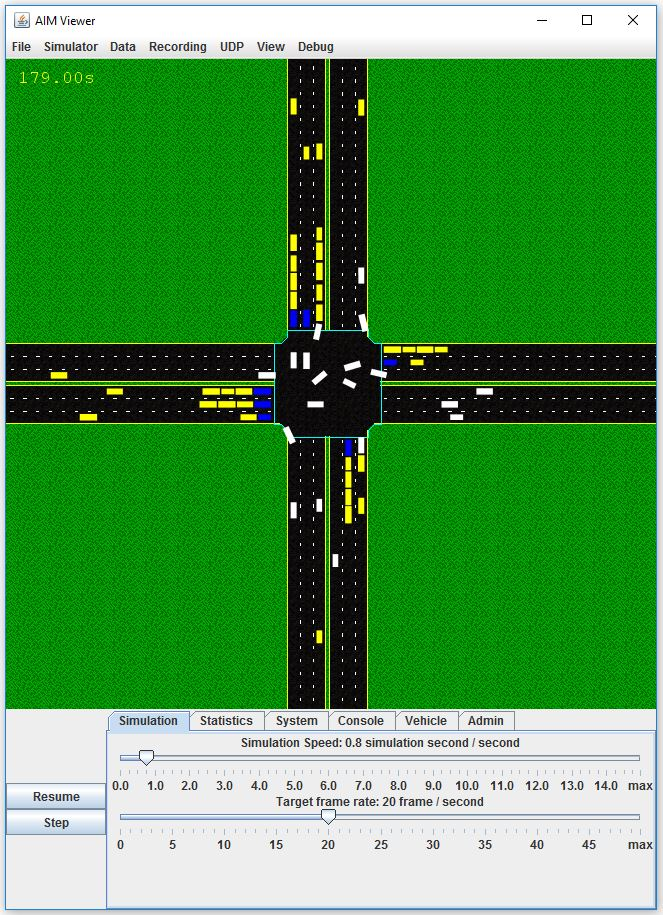
\includegraphics[width=\textwidth]{AIMOriginal.JPG}
\caption{Screenshot of the AIM Simulator}
\label{fig:AIMOriginal}
\end{figure}

A grid-based reservation system works well in high traffic zones like intersections, because it forces all vehicles to communicate with a single entity. This entity has a global-view of activity at the junction, allowing the system to make vehicle management decisions more easily. A V2V solution would require more complex communication protocols involving large numbers of vehicles. The volume of messages required for each vehicle to obtain a global view of the intersection would be considerably larger, and as such, most vehicles will never get a complete understanding of the status of the intersection.

A centralised system for lane changing was described in a paper by Atagoziyev et al. in 2016 \citep{Atagoziyev2016}. This system uses roadside infrastructure to help groups of vehicles change lanes before they reach a 'critical-position', such as a motorway exit or intersection. The vehicles send their position and velocity information to the roadside infrastructure; the system then sends a number of orders to the vehicles such that they safely rearrange themselves into the correct lanes.  Because the distance travelled by the vehicles involved can be large, particularly at high speeds, the system would struggle to use a reservation tile based system as AIM did, instead Atagoziyev's system manages the gaps between vehicles to safely relocate vehicles into the correct position. A more comprehensive overview is given in \ref{subsec:Lane Changing to hit a target lane}.

Atagoziyev's system would only need to be applied during the approach to critical-positions. Vehicles could be managed using platoons or another vehicle following model until that point. A centralised system provides a single communication point which manages all of the vehicles that want to change lanes. This helps to reduce the volume of communications required and creates an entity with a global view of the vehicles' positions and goals. A V2V solution would most likely require more communications and may never obtain a complete picture of the situation, possibly leading to sub-optimal lane changing orders.

Note that Atagoziyev's system could be adapted, such that all of the vehicles communicate with the platoon leader instead of roadside infrastructure. Though this could be called a V2V communication solution, the effective solution is still considered centralised, as all decisions are made by one entity.

\subsection{Decentralised Systems}
\label{subsec:Decentralised Systems}
The main arguments against centralised systems generally tend to stem from concerns over feasibility and fault tolerance. A centralised V2I solution relies on one system always being available to manage vehicles. The original implementation of the AIM system works well, but if the system were to fail and no longer provide reservations then approaching vehicles will simply halt at the intersection. In a worst case scenario, the system would still give reservations, but fail to compare them to reservations already in place, causing major car crashes in the intersection. Having, a single point of failure (SPOF) like this is a major concern, particularly when lives are on the line.

A paper by Van Middlesworth et al. in 2008 \citep{VanMiddlesworth2008} defined a decentralised version of the AIM model using V2V communication protocols. 

In Van Middlesworth model each vehicle can broadcast two different types of message. These messages are broadcast repeatedly with a specified period.
\begin{enumerate}
\item CLAIM
This is a message indicating the vehicle's intention to traverse the intersection. It provides the vehicle's VIN, arrival lane, turning direction, arrival time and exit time. It also provides a message id, which increments when a new message is broadcast. Finally, the CLAIM message contains a boolean indicating whether the vehicle has stopped at the intersection.
\item CANCEL
This message releases any currently held reservation, it contains the vehicle's VIN and a message id, which acts the same as the message id in CLAIM.
\end{enumerate}

Two CLAIM messages are in conflict if their paths, as determined by their lane and turn parameters, are incompatible and their time intervals, as determined by their arrival and exit times, overlap. To resolve the conflict Van Middlesworth defines a priority ordering over claim messages using the following rules:
\begin{enumerate}
\item If neither vehicle is stopped at the intersection, the claim with the earliest exit time has priority.
\item If both vehicles are stopped, the vehicle whose lane is 'on the right' has priority. This is defined similarly to current US 4-way stop rules.
\item If neither lane can be considered to be on the right the vehicle who is not making a turn has priority.
\item If no other priority order can be established, the vehicle with the lowest VIN has priority.
\end{enumerate}

The protocol starts with approaching vehicles receiving messages from existing pending vehicles. An approaching vehicle may not start broadcasting it's own messages until it is within 'lurk distance' of the intersection. 

Once within lurk distance the vehicle tries to make a reservation using a CLAIM message. The vehicle will continue generating CLAIM messages, searching for an available time block, increasing and decreasing its velocity as necessary, until it finds one that allows it to traverse the intersection without any other CLAIM having priority over it.

Once the vehicle has a CLAIM broadcasting it may need to change it if it's looking like the vehicle might be late to the intersection or if a competing CLAIM arrives with a higher priority. A vehicle might also change its CLAIM to take advantage of a newly available time slot. In this situation the vehicle must then send a CANCEL message and a new CLAIM. Once the vehicle reaches the intersection it must traverse according to its current CLAIM, broadcasting its CLAIM throughout the traversal. At this point, the vehicle has the highest priority CLAIM and cannot be interrupted.

The main drive behind the unmanaged AIM intersection was to reduce cost. Adding in new infrastructure to an intersection costs money, and it might not be considered worthwhile for small intersections with only one or two lanes on each side. An unmanaged, decentralised system like that described by Van Middlesworth would drastically reduce the cost to the state in creating automated road networks.

Cost also becomes a major issue for centralised systems when you consider fast moving situations such as lane changing on a motorway. To implement Atagoziyev's model, vehicles must remain in range of the roadside infrastructure. This would mean that the infrastructure will have to continue on for a long distance, which could become very expensive, especially given the number of critical-positions on a motorway. Decentralised solutions reduce these costs massively.

Two examples of decentralised lane changing models are Gipps' 1986 driver decision model \citep{Gipps1986} and the MOBIL model developed by Kesting et al. in 2007 \citep{Kesting2007}. These models are decentralised and as such do not have to rely on roadside infrastructure in order to change lanes. This greatly reduces the cost of both implementations and allows the vehicles to be more flexible as to when they change lanes, no longer having to wait until they reach the lead up to a critical-position supported by roadside infrastructure. This flexibility means that vehicles could change lanes to increase their average velocity rather than just changing lanes in order to make a turn or leave the motorway at a critical-position. It also allows vehicles to deal with unexpected situations far from any roadside infrastructure. For example, a broken down car blocking a lane can be evaded. There is more information on Gipps' 1986 model and MOBIL in \ref{sec:Making lane changing decisions}.

\section{Making lane changing decisions}
\label{sec:Making lane changing decisions}
There are a number of reasons that a driver would want to change lanes. The most obvious being that the journey the driver wishes to complete requires the vehicle to move into a different lane. In this case the vehicle \emph{must} change lanes before it reaches a critical position. Beyond this position the driver will need to change their planned route, most likely extending their journey time. 

Another reason a driver might change lanes is in order to increase velocity, with the aim of reducing journey time. In general, a driver will aim to change lanes if their average velocity in their current lane is much less than that the velocity it could be achieving in another lane.

\subsection{Lane Changing to hit a target lane}
\label{subsec:Lane Changing to hit a target lane}
In 1986 Gipps' modelled driver behaviour in real world circumstances, characterising the decisions a driver has to make in order to determine whether to change lanes \citep{Gipps1986}. The paper was designed to be used with the Gipps' 1981 car-following model \citep{Gipps1981}, explained in \ref{sec:Car Following Models}.

The model itself is constructed as a flow chart, in which the decision nodes are the choices a driver must make. \newtext{You can see the flowchart in Figure \ref{fig:Gipps1986Flowchart}}.

\begin{figure}[htb]
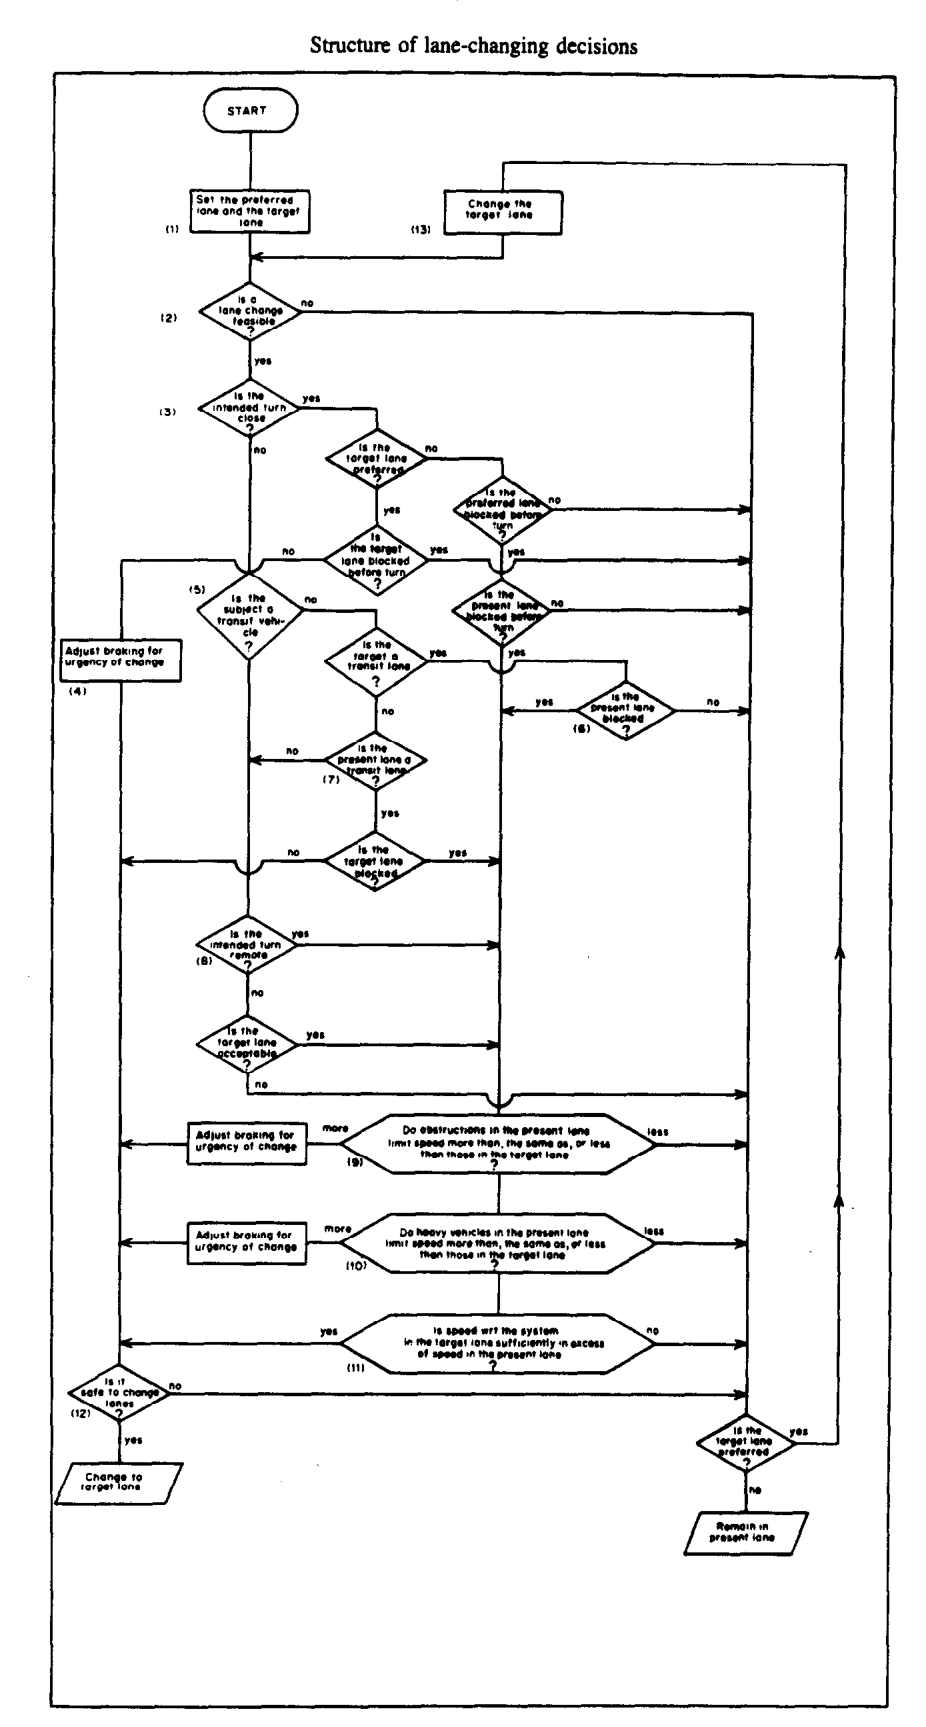
\includegraphics[width=\textwidth]{Gipps1986Flowchart.png}
\caption{The flowchart for lane changing decisions from \citep{Gipps1986}}
\label{fig:Gipps1986Flowchart}
\end{figure}

After determining whether a lane change is feasible the model considers whether the driver needs to move into another lane because they are heading towards a critical point.

These decisions are modelled in nodes 3 and 4.

\begin{enumerate}
\item[3] \textit{Driver behaviour close to the intended turn}

If the driver is close to their intended turn then they will always attempt to change into their preferred lane. Only if blocked will they consider moving into another lane. 

'Close' varies depending on regional differences and the level of traffic, but in the model, close is defined as the driver being within a distance equal to ten seconds of travel from the turn at the driver's desired speed.

\item[4] \textit{Urgency of changing lanes}

The urgency of changing lanes increases as the driver gets closer to their turn. The willingness of the driver to brake harder and accept smaller gaps increases as the driver gets closer to their intended turn.

In the implementation, the braking rate a driver is willing to when first becoming close doubles by the time the intended turn is reached. 

\begin{itemize}
\item[$D_n$] is the location of the intended turn
\item[$V_n$] is the desired (or free) speed of the driver
\item[$b_n^*$] is the most severe braking the driver would otherwise be willing to undertake
\end{itemize}

\begin{equation}
b_n = \Biggl[2 - V_n\frac{(D_n - x_n(t))}{10}\Biggr]b_n^*
\end{equation}

\end{enumerate}

Similarly to Gipps 1981 car-following model, this driver decision model is based on human driver behaviour and as such falls into similar pitfalls. There could be more optimal driver behaviours which would ensure that a driver is in the correct lane well before the critical position. However, because Gipps 1986 model is designed to model human driving behaviour we can expect it to perform less than optimally.

\newtext{Atagoziyev's model is designed around autonomous vehicles, which allows it to take advantage of vehicle-to-vehicle communication}. The model manages a set of vehicles over two lanes, organising their movements into their preferred lanes before they reach a critical position.

To do this the model keeps track of the gaps between vehicles and their relative speeds using roadside infrastructure. Then, a series of equations, each describing a different situation, are used to determine the behaviour of the vehicle.

In the paper SV (subject vehicle) refers to the vehicle that wants to change lanes. CL (current lane) is the vehicle in front of the SV. TL (target lane) is the vehicle the SV wants to be behind in its target lane. LV (lag vehicle) is the vehicle that will be behind SV once it moves to its target  lane. \newtext{Atagoziyev defines seven equations for manipulating vehicles between lanes. They are used in different contexts, each based on the relative positions of the surrounding vehicles. The contexts for each equation are given below, along with the behaviour from the equation during that context.}

\begin{enumerate}
\item[Case 1] \textit{SV too close to CL in its current lane or TL if it changed lanes.}

SV slows down until the gap is sufficiently large enough.
\item[Case 2] \textit{SV has a large gap between itself and TL and CL, however, LV is too close to SV}

SV can approach CL and TL as long as the gap remains large enough. LV needs to open up a sufficient gap behind SV.
\item[Case 3] \textit{SV has the minimum allowable gap to TL and CL, but LV is too close}

SV follows the closest leader and waits until LV creates the necessary gap.
\item[Case 4] \textit{The gaps between SV and CL/TL/LV are sufficient. But CL/TL are not travelling at the 'nominal speed' established for all vehicles in this exchange}

SV maintains a sufficient gap, waiting for CL/TL to travel at nominal speed again.
\item[Case 5] \textit{SV and CL/TL/LV have sufficient gaps and CL/TL are travelling at nominal speed.}

SV performs the lane change, maintaining nominal speed.
\item[Case 6] \textit{SV obtains the minimum gap to CL/TL and LV maintains a sufficient gap. CL/TL are not travelling at nominal speed}

SV maintains the minimum gap, waiting for CL/TL to travel at nominal speed again.
\item[Case 7] \textit{SV obtains the minimum gap to CL/TL and LV maintains a sufficient gap. CL/TL are travelling at nominal speed}

SV performs the lane change, maintaining nominal speed.
\end{enumerate}

These equations are the building blocks that lead to a lane change. \newtext{The flowchart in Figure \ref{fig:AtogoziyevFlowchart} shows how they work together to enact a single lane change.}

\begin{figure}[htb]
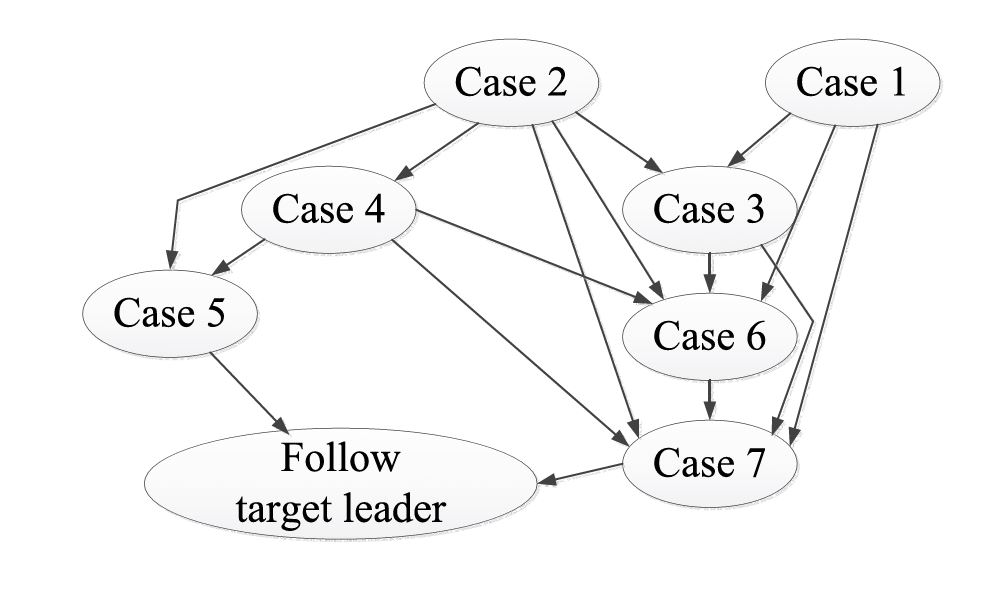
\includegraphics[width=\textwidth]{AtagoziyevFlowchart.JPG}
\caption{The flowchart for Atagoziyev's Lane Changing model equations}
\label{fig:AtogoziyevFlowchart}
\end{figure}

Using this algorithm, we can move multiple vehicles into their correct lanes. LV always provides space to allow each changing vehicle into the correct lane. All of the vehicles are working with each together, such that they can all reach their goal. Comparing this to Gipps' 1986 model, where drivers are acting solely in their own interest, we can see that by having an external agent managing lane changes, the autonomous vehicles can achieve results that might not be possible in situations where drivers are acting selfishly. For example, in a grid locked situation, drivers following Gipps' model might never be able to move into their desired lane; however vehicles following Atagoziyev's model would open up spaces allowing vehicles to move through the traffic.

\subsection{Lane Changing to improve overall velocity}
\label{subsec:Lane Changing to improve overall velocity}
Gipps' driver decisions model also considered situations where the driver does not have to be in any particular lane. The model considers the effects of transit lanes, heavy vehicles and the effect of the preceding vehicle on the driver's vehicle. \newtext{These are shown in nodes 5 to 7 and 9 to 11 of Gipps' flowchart in Figure \ref{fig:Gipps1986Flowchart}}.

\begin{enumerate}
\item[5] \textit{Transit vehicles and lanes}
Transit lanes are lanes dedicated solely for public transport and other high occupancy vehicles. These include vehicles such as buses, taxis and carpool cars. These vehicles are known in the model as 'transit vehicles'.
\item[6] \textit{Entry of nontransit vehicles into transit lanes}
If there is an obstruction in the present lane, it is often considered to be a valid reason for a non-transit vehicle to enter a transit lane. 
\item[7] \textit{Departure of nontransit vehicles from a transit lane}
Once the obstruction has been cleared, nontransit vehicle must move back into a valid lane. This forced departure does not affect vehicles that are close to their intended turn.
\item[9] \textit{Relative advantages of present and target lanes}
If the driver has not yet been forced to change lanes by any other factors, then they can look at the relative advantages of the present and target lanes, considering obstructions and then determining which lanes obstructions will have the least effect on their safe speed.
\item[10] \textit{The effect of heavy vehicles} 
If obstructions are level with each other or beyond the range a driver considers, then the driver considers the next heavy vehicle in each lane, as if it were the leading vehicle in an ordinary car following situation. The driver then selects the lane which will give them the higher speed.
\item[11] \textit{The effect of the preceding vehicle}
If there are then no heavy vehicles, the driver considers the speed possible in each lane and then changes if they gain a 'sufficient' speed advantage. This is again, subjective, depending on the present lane, target lane and the type of vehicle.
\end{enumerate}

Again, Gipps' 1986 model was built with human drivers in mind, and as such it fails to take advantage of the benefits of autonomous vehicles \newtext{such as platooning and vehicle-to-vehicle communications.}

Work by Kesting et al. in 2007 \citep{Kesting2007} describes a decentralised model of lane changing that lets vehicles change lanes to increase velocity whilst still ensuring that the overall traffic flow is not disrupted. This helps to avoid traffic shocks and maintains smooth traffic flow. \newtext{In order to do this, Kesting introduces the MOBIL or 'Minimising Overall Braking Induced by Lane Changes' model. The model uses two criterion that the vehicle must satisfy.}

\newtext{
The first criterion deals with safety, ensuring that the deceleration of a successor vehicle $\tilde{a}_n$ in the target lane doesn't exceed a safety limit $b_{safe}$.
}

\begin{equation}
\tilde{a}_n \geq -b_{safe}
\end{equation}

This criterion effectively puts a limit on the level of braking a vehicle changing lanes can cause another vehicle to undergo if it pulls out in front of it.

The second criterion is the 'incentive criterion' which is what motivates a driver to change lanes. This criterion introduces a 'politeness factor' $p$ which expresses the extent to which nearby vehicles affect a driver's lane changing decision. 

\newtext{
The paper discusses the differences between symmetric ('US') lane changing rules and asymmetric ('European') passing rules, however in this paper we only use US lane changing rules. This gives the incentive criterion:
}

\begin{equation}
\underbrace{\tilde{a}_c - a_c}_\text{driver} + p(\underbrace{\tilde{a}_n  - a_n}_\text{new follower} + \underbrace{\tilde{a}_o - a_o}_\text{old follower}) > \Delta a_{th}
\end{equation}

$\tilde{a}_x - a_x$ is the utility a driver x gets due to the lane change, where $\tilde{a}_x$ is the acceleration of vehicle x after the lane change and $a_x$ was their acceleration before the lane change. $c$ is the vehicle changing lanes, $n$ is the vehicle behind $c$ once it changes lanes, and $o$ is the vehicle following $c$ before the lane change. $\Delta a_{th}$ is the threshold at which the driver will change lanes. It is designed to model inertia. A driver won't change lanes unless they get above a specific utility gain. The politeness factor $p$ varies from $0$ to $1$, where $p = 0$ is the most selfish behaviour and $p = 1$ describe drivers who won't change lanes unless collectively all of the drivers gain a utility greater than the threshold. When $p > 1$ drivers won't change lanes at all if it negatively affects the surrounding traffic, drivers will even go so far as to execute lane changes which reduce their own utility. Likewise drivers with $p < 0$ will go out of their way to negatively affect other drivers, even reducing their own utility to do so.

The idea of a MOBIL model means that drivers will only change when it increases the sum of all of the accelerations increases. This would be at $p = 1$ and $\Delta a_{th} = 0$. In this case the equation becomes 

\begin{equation}
\tilde{a}_c + \tilde{a}_n + \tilde{a}_o > a_c + a_n + a_o 
\end{equation}

\newtext{
Kesting found that the most important parameter affecting the rate of lane changing was $p$. With a $p$ value of 1 the maximum lane changing rate was almost halved. Kesting also discovered that 'altruistic' lane changing behaviour increased the mean speed of both lanes involved in the simulation, improving overall traffic performance.
}

\newtext{
Comparing this to Gipps' 1986 approach we can see that MOBIL is far more considerate of other drivers and as such the overall speed of the vehicles on the road could be higher. MOBIL is also designed for autonomous vehicles, which allows it to enforce 'altruistic' behaviour from vehicles on the road. The model could also be extended to include V2V communications. Transmitting accurate braking profiles to other vehicles would make it easier to determine the effect a lane change would have on the overall system.
}
\chapter{Problem Analysis}
\label{cha:Problem Analysis}
Lane merging is not a straightforward problem with a single solution. There are many different types of lane merging scenarios as well as a number of factors which add more variance to the problem. Section \ref{sec:Merge Types} analyses some of the different merging scenarios to better define them. Section \ref{sec:Measuring Success} indicates how success of a merge scheme can be measured and Section \ref{sec:Merge Variance Factors} defines some factors that could alter the behaviour of a given merge scenario.

\section{Merge Types}
\label{sec:Merge Types}
In this paper we focus on merges made at `critical positions' such as junctions. This is true for all of the merge scenarios analysed. Figure \ref{fig:laneCollection} illustrates some of the merge scenarios described.

\begin{figure}
\centerline{
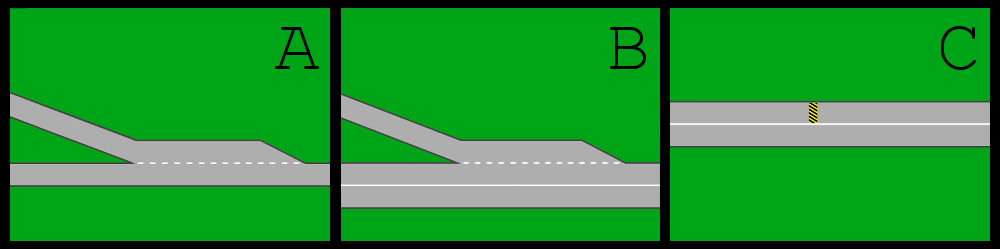
\includegraphics[width=14cm]{laneDiagrams/laneCollection.png}
}
\caption{a) S2S with slip lane, b) S2D with slip lane, c) Lane obstruction}
\label{fig:laneCollection}
\end{figure}

\subsection{Single-to-Single Merge}
\label{subsec:Single-to-Single Merge}
A single-to-single merge (S2S merge) describes a situation where a vehicle moves from a single lane road into another single lane road. In this situation we label the lane that vehicles are moving from, the `merge lane' (ML), and we label the lane that vehicles move to, the `target lane' (TL). The vehicles on the TL generally tend to be faster moving. We describe the vehicles that start on the ML as `merging vehicles' (MVs) and the vehicles that start on the TL as `TVs' (TVs). We have our critical position where the ML and TL intersect. We call this area the `merge zone'.

The main issue with an S2S merge stems from the limited options available to vehicles arriving at the critical position. Target vehicles do not have the opportunity to move laterally out of the way of MVs, and vehicles on both lanes could struggle to reduce their velocity without affecting their successors.

Many S2S merges are performed with an attached slip-road. A slip-road gives MVs more time to travel parallel to the TL before merging. This makes the merge easier for both MVs and TVs as MVs don't slow down in front of TVs in order to make the turn into the TL. Figure \ref{fig:laneCollection} A shows an S2S Merge with a slip lane.

\subsection{Single-to-Double Merge}
\label{subsec:Single-to-Double Merge}
A single-to-double merge (S2D merge) describes a situation where a vehicle moves from a single lane road into a double lane road. In this situation we have two TLs. The upper lane which directly links to the merging lane is called 'target lane 1' (TL1) and the lower lane is called 'target lane 2' (TL2). We still have only one critical position where the merging lane meets TL1.

An S2D merge provides more options for vehicles on the targets lanes at the critical position. Target vehicles now have the opportunity to move laterally to avoid MVs. Two lanes also allows for more vehicles on the TL which should give vehicles greater freedom to adjust their velocity without affecting their successors, at least when compared to the same number of vehicles on a single lane.

S2D merges can also take advantage of a slip-road. Figure \ref{fig:laneCollection} B shows an S2S Merge with a slip lane.

\subsection{Lane Obstruction Merge}
\label{subsec:Lane Obstruction Merge}
A lane obstruction merge is where a vehicle needs to change lanes to avoid an obstacle in their way. It is essentially an S2S merge although the vehicle moves laterally to avoid the obstacle. In this situation the critical position is a point shortly before the obstruction. 

The obstacle could be a broken down vehicle or some debris on the road. Because of the unexpected nature of the obstacle it may sometimes be difficult to have a centralised approach to the problem. Although, if the obstacle was a broken down vehicle, the vehicle might be able to act as the centralised system managing approaching vehicles. Figure \ref{fig:laneCollection} C shows an a lane obstruction merge scenario.

\section{Measuring Success}
\label{sec:Measuring Success}
In order to evaluate the effectiveness of solutions to the problems we need to define measurements of success. 

Solutions to the merging problems above must satisfy the following conditions:

\begin{enumerate}
\item \textit{No collisions}
This means avoiding collisions at the critical position between MVs and TVs, as well as avoiding collisions between vehicles on the same lane.
\item \textit{Minimise delays to both lanes}
Vehicles should not suffer large delays to travel time due to the merge. This means measuring average delay for both the ML and TL to ensure that the system is not starving one lane for the benefit of vehicles on the other.
\item \textit{Maximise throughput}
By minimising delays and velocity loss we aim to maximise the throughput of the critical position.
\item \textit{Minimise changes in velocity}
Though not strictly a performance requirement, the system should minimise changes in vehicle velocity, for both passenger comfort and vehicle efficiency.
\end{enumerate}

We need to measure how well solutions meet these conditions. 

\subsection{Collisions}
\label{subsec:Collisions}
Preventing collisions is a basic safety requirement for any autonomous vehicle system. We can measure this by comparing the positions of vehicles in the system, and ensuring that there is no overlap.

We should also consider measuring near misses. We can define a minimum spacing between vehicles, perhaps equal to the minimum braking distance of the vehicle plus an additional comfort distance. This would mimic the IDM model \citep{Treiber2000}.

Any collisions that do happen should be reported immediately. The system should automatically be considered a failure.

\subsection{Delay}
\label{subsec:Delay}
Delay measures the effect that the critical position had on the overall journey of the vehicle. It is the primary metric considered in Dresner et al.'s 2004 paper \citep{Dresner2004} on AIM.

Dresner et al. provide the following equation for measuring average delay.

\begin{equation}
\frac{1}{|C|}\sum_{v_i\in{C}}\bigl(t(i) - t_0(i)\bigr)
\end{equation}

$C$ is the set of vehicles that pass through a critical position within a set time frame. Assuming no other vehicles on the road, a vehicle $v_i$ would complete it's trip in time $t_0(i)$, otherwise $v_i$ would complete it's trip in time $t(i)$. We can represent this trip for vehicles in the simulator as the time difference between the vehicle spawning in and the vehicle being removed from the simulator.

To ensure fairness the mean delay will be measured across each lane.

\subsection{Throughput}
\label{subsec:Throughput}
By minimising delay we should also maximise throughput; the two are closely related. However we should also collect direct metrics.

\begin{equation}
\text{Vehicle throughput} = \frac{|C|}{t}
\end{equation}

Here $t$ is the time it took for all of the vehicles in $C$ to pass through the critical position. We will also need throughput measurements for each lane separately.

\subsection{Velocity Changes}
\label{subsec:Velocity Changes}
Vehicles should aim to reduce velocity changes as much as possible, particularly rapid changes. Ideally autonomous vehicles should have very smooth acceleration and braking profiles. This both increases passenger comfort and improves fuel efficiency. To measure maximum acceleration and deceleration we can measure the change in velocity at each time step in the simulator, and divide this change by the time-step length.

\section{Merge Variance Factors}
\label{sec:Merge Variance Factors}
In each of the scenarios in section \ref{sec:Merge Types} the road layout is fixed. More variance can be introduced to the scenarios by altering other factors. Not all of the factors below will be applicable in every merge scenario. Figure \ref{fig:s2sMarked} shows some of the factors below, applied to an S2S merge.

\begin{itemize}
\item \textit{Traffic Level} 
The traffic level changes the traffic density. It is measured in vehicles per hour per lane (\si{vhl})
\item \textit{Target lane speed limit}
The maximum speed that vehicles on the target lane can travel.
\item \textit{Merge lane speed limit}
The maximum speed that vehicles on the merge lane can travel.
\item \textit{Target lane lead in distance}
The distance between the point at which TVs arrive in the simulation and the point at which the TVs reach the merge zone.
\item \textit{Target lane lead out distance}
The distance between the end of the merge zone and the end of the target lane (at least the end in the simulator).
\item \textit{Merge lane lead in distance}
The distance between the point at which MVs arrive in the simulation and the point at which the MVs reach the merge zone.
\item \textit{Merging angle}
The interior angle $\theta$ at the point where the merging lane meets the target lane.
\item \textit{Slip-road length}
The length of the slip-road in a merge that uses a slip-road.
\end{itemize}

\begin{figure}[htb]
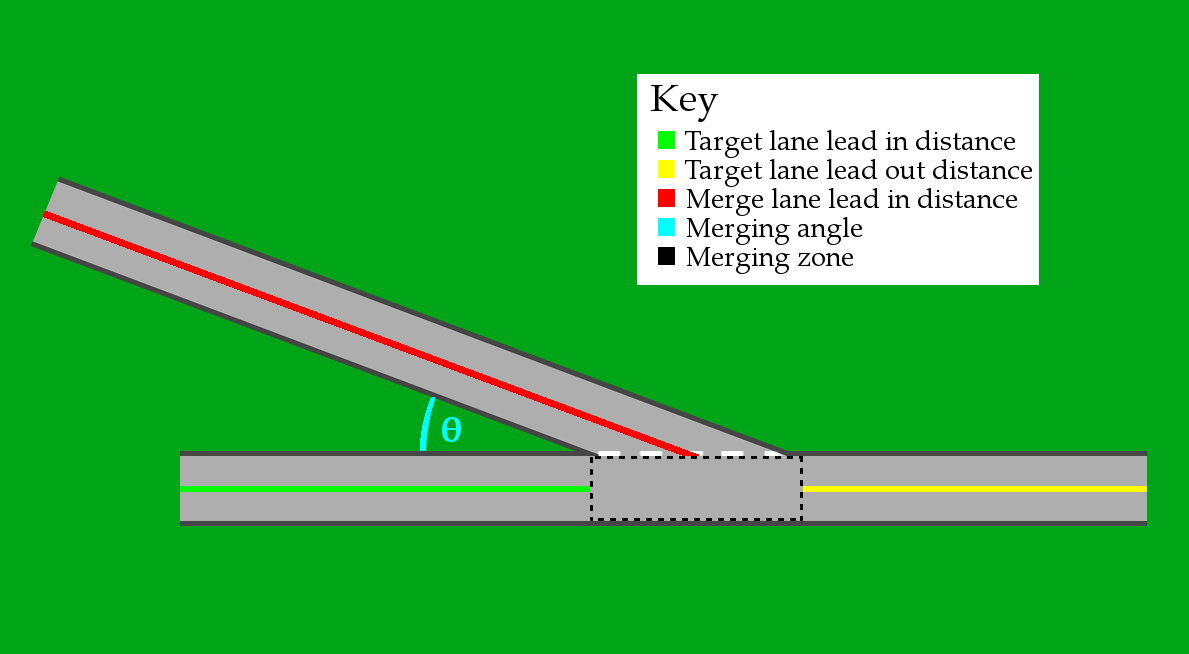
\includegraphics[width=\textwidth]{laneDiagrams/s2sMarked.png}
\caption{An S2S merge marked with some of the variance factors}
\label{fig:s2sMarked}
\end{figure}

Traffic level has a fairly obvious effect on performance in a particular merge scenario. The more vehicles that try to merge together the more difficult it will be for the merge to happen. It will likely require vehicles to move more slowly. Increased traffic density also increases the likelihood of traffic shocks, and vehicle manoeuvrability is impacted.

Altering speed limits could also affect performance. Higher speed limits could put pressure on systems that process the vehicles. Vastly differing speed limits for each lane could impact how easily a vehicle finds it to merge into another lane, and adapt to its speed limit.

Lead in distances change the amount of deliberation time vehicles have before they reach the junction. It also changes the distance they have to change their velocity in. This means that shorter distances could lead to larger acceleration and deceleration values as well as sub-optimal solutions to the merge. 

The merging angle changes the heading at which MVs arrive, but also the length of the merge zone. This could impact how long it takes a vehicle to traverse the merge zone as well as affecting how easily the vehicles adjust to the new lane heading.

\section{Requirements}
\label{sec:Requirements}
Using the problem analysis above, we can define requirements for our final system. This system will not deal with every merge scenario described but will instead set the groundwork for further research. The complete requirements are given in Appendix \ref{sec:RequirementsAppendix}. A shortened version with the most important requirements are given here.

\subsection{Functional Requirements}
\label{subsec:Functional Requirements}
The functional requirements describe the functionality required within the simulator. They are broken into two sets of requirements. User requirements and system requirements. User requirements describe the behaviour expected from the simulator from a user perspective. System requirements are all associated with a user requirement. They describe the functionality required by the system in order to satisfy the user requirement. Table \ref{tab:functionalRequirements} shows some of the functional requirements.

\begin{longtable}{|p{0.1\linewidth}|p{0.4\linewidth}|p{0.1\linewidth}|p{0.4\linewidth}|}
% Headings and Footers %
\caption{Functional requirements table.}\label{tab:functionalRequirements}\\
\hline
\multicolumn{2}{|l|}{User Requirements} & \multicolumn{2}{l|}{System Requirements} \\
\hline
\endfirsthead

\hline
\multicolumn{2}{|l|}{User Requirements} & \multicolumn{2}{l|}{System Requirements} \\
\hline
\endhead

\hline
\endfoot

\hline
\endlastfoot

% Data %

FU.3 & Users can run merge simulations. & FS.13 & The system can run merge simulations \\
\hline
FU.5 & User can view the activities of a simulation. & FS.51 & The system displays the current status of a simulation as it runs. \\
\hline
\multirow{2}{*}{FU.6} & \multirow{2}{*}{\parbox{\linewidth}{Users can export the results of a merge simulation.}}
 & FS.61 & The system has controls for exporting results data. \\
 &  & FS.62 & The system can produce a file containing results data from the simulation. \\
\hline
FU.7 & Users can select and run an S2S merge simulation. & FS.71 & The system can produce S2S simulations. \\
\hline
FU.8 & Users can select a centralised merging scheme with S2S merge simulations. & FS.81 & The system can use an AIM-like merge management system for the merging zone in an S2S simulation. \\
\hline
FU.9 & Users can select a decentralised merging scheme with S2S merge simulations & FS.91 & The system can use an merge management scheme similar to that described in \citetitle{VanMiddlesworth2008} \citep{VanMiddlesworth2008}. \\
\hline
FU.16 & Users should be alerted of any collisions during a simulation. & FS.161 & The system should be able to alert the user if a collision occurs. 
\end{longtable}

\subsection{Non-functional Requirements}
\label{subsec:Non-functional Requirements}
The non-functional requirements describe the expectations of the simulator that are not actions the simulator will perform. Table \ref{tab:nonFunctionalRequirements} shows some of the non-functional requirements for the simulator.

\begin{longtable}{|p{0.1\linewidth}|p{0.9\linewidth}|}
% Headings and footers %
\caption{Non-functional requirements table.}\label{tab:nonFunctionalRequirements}\\
\hline
ID & Description \\
\hline
\endfirsthead

\hline
ID & Description \\
\hline
\endhead

\hline
\endfoot

\hline
\endlastfoot

NS.6 & All data displayed to the user should be accurate. \\
\hline
NS.7 & All data in the results file should be accurate. \\
\hline
NS.9 & Code should be written to allow for easy expansion. \\
\hline
NS.11 & The simulator should be integrated into the AIM4 simulator without negatively affecting the performance of AIM simulations. \\
\end{longtable}
\chapter{Design}
\label{cha:Design}

\section{S2S}
\label{sec:S2S}
The S2S merge is the simplest of those described in Chapter \ref{cha:Problem Analysis}. Any merging system must perform well in the S2S merge before being developed further to tackle more complex merge problems.

\subsection{Map}
\label{subsec:Map}
In order to build the map using the user's parameters we will need to calculate the relative positions of the lane entrances and exits as well as the locations of the data collection lines and spawn points.

To start with, we need to calculate the dimensions of the merging zone. The height of the merging zone will be the same as lane width of the target lane. The length can be calculated using the right-angled triangle in Figure \ref{fig:mergingZoneTriangle}. Using this triangle and some trigonometry we can calculate the length of the merge zone ($h$ in Fig. \ref{fig:mergingZoneTriangle}) using equation \ref{hSin}.

\begin{figure}[htb]
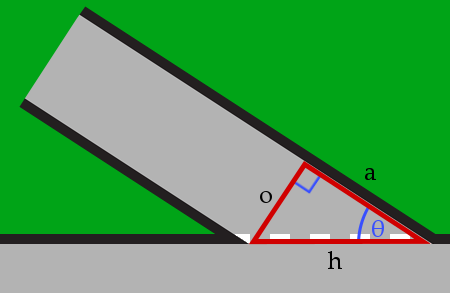
\includegraphics[width=\textwidth]{designNotes/mergingZoneTriangle.png}
\caption{A right-angled triangle used to calculate the size of the merging zone.}
\label{fig:mergingZoneTriangle}
\end{figure}

\begin{equation}\label{hSin}
h = o / \sin(\theta)
\end{equation}

We also need to know whether the horizontal width of the merge lane on the map, or it's 'base width' is longer than the target lane's lead in distance, plus the merge zone length. This will determine the width of the overall map, as if the merge lane's base length is longer then the target lane will not start with co-ordinate $x=0$ as it would if the target lane determined the width of the map.

Firstly we need to calculate the X and Y adjustments at the merge lane entrance. Because the vehicles drive in the centre of the lane and the merge lead in distance is defined by the middle line of the lane we still need to calculate how far the lane extends in the x and y directions due to it's width. To do this we can use the right-angled triangles shown in Figure \ref{fig:mergeEntranceTriangles}

\begin{figure}[htb]
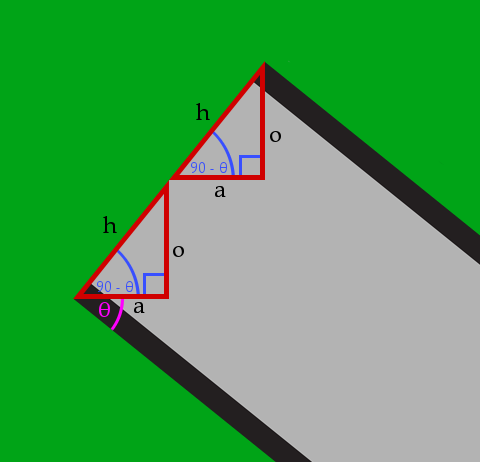
\includegraphics[width=\textwidth]{designNotes/mergeEntranceTriangles.png}
\caption{Two right-angled triangles used to calculate the x and y adjustments for the merge entrance.}
\label{fig:mergeEntranceTriangles}
\end{figure}

These triangles have the same dimensions and have an interior angle of 90 - $\theta$ due to the 'alternate angle' or 'z-angle' rule. Each triangle has a hypotenuse with a length equal to half the width of the lane. 

The x-adjustment for the merge entrance is the length of the adjacent side of one of the lower triangle and the y-adjustment for the merge entrance is the length of the opposite side of the upper triangle (though both triangles do have the same dimensions). We can use equation \ref{aCos90} to calculate the X-adjustment and equation \ref{oSin90} to calculate the Y-adjustment.

\begin{equation}\label{aCos90}
a = h \cos(90 - \theta)
\end{equation}{}

\begin{equation}\label{oSin90}
o = h \sin(90 - \theta)
\end{equation}

To calculate the 'base width' of the merge lane we will also need to calculate the adjacent side of the triangle in Figure \ref{fig:baseWidthTriangle}. In this triangle the hypotenuse has a length equal to the merge lead in distance. Therefore, we can use equation \ref{aCos} to calculate the length of the adjacent side. After obtaining the length of this side we simply add the merge entrance X-adjustment and half the length of the merge zone to find the merge base width.

\begin{figure}[htb]
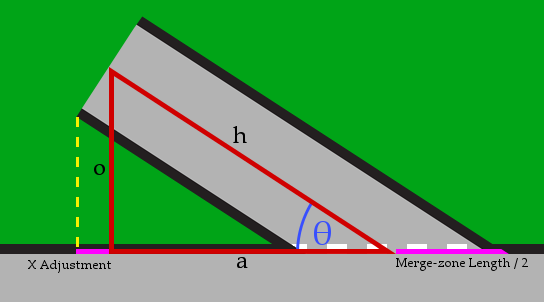
\includegraphics[width=\textwidth]{designNotes/baseWidthTriangle.png}
\caption{A right-angled triangle used to help calculate the base width of the merge lane, along with the X-adjustment and merge-zone length.}
\label{fig:baseWidthTriangle}
\end{figure}

\begin{equation}\label{aCos}
a = h \cos(\theta)
\end{equation}

We also need to find the point at which the merging lane's centre line crosses the target lane's centre line in the merge zone. We know the Y-coordinate for this point as it will be the same as the Y-coordinate of the target lane centre line. We also know the X-coordinate of the point at which the merge lane's centre line meets the target lane. We can use these two co-ordinates to create the triangle shown in Figure \ref{fig:toCentreTriangle}. We can then use equation \ref{aTan} to find the X-adjustment from the merge zone centre to the point where the two centre lines cross.

\begin{figure}[htb]
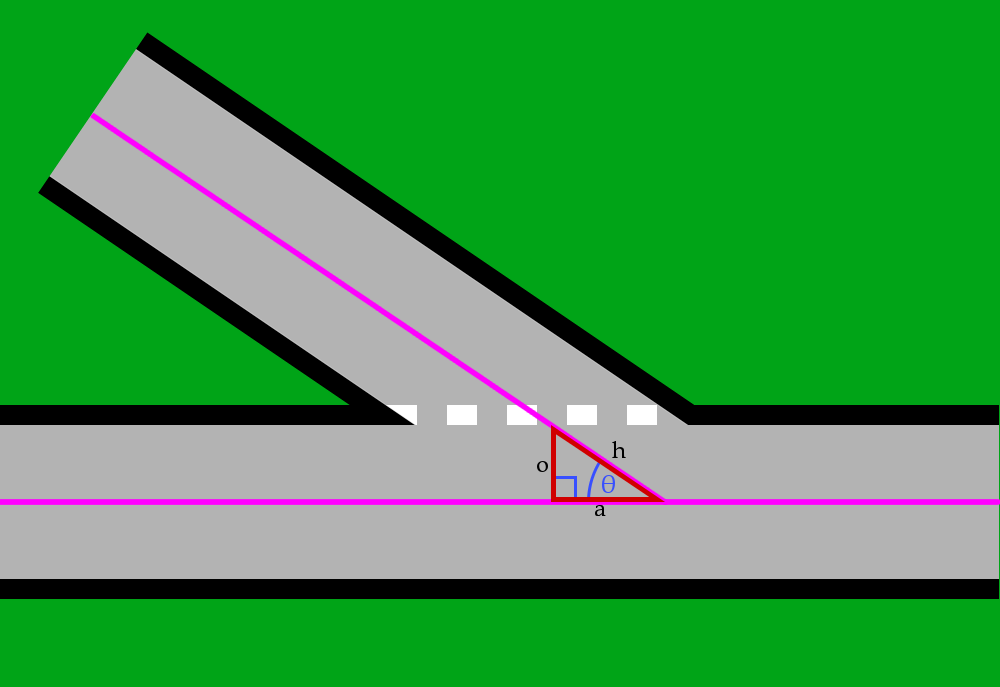
\includegraphics[width=\textwidth]{designNotes/toCentreTriangle.png}
\caption{A right-angled triangle used to calculate where the two centre lines meet. The centre lines are indicated in pink.}
\label{fig:toCentreTriangle}
\end{figure}

\begin{equation}\label{aTan}
a = o / \tan(\theta)
\end{equation}

\subsection{Intersection Management System}
\label{subsec:Intersection Management System}

\subsection{Decentralised Communication System}
\label{subsec:Decentralised Communication System}

\subsection{Measuring Success}
\label{subsec:Measuring Success}

\chapter{Implementation}
\label{cha:Implementation}
The final implementation was done in Java, an was built on top of the AIM simulator codebase. All class diagrams were created using IntelliJ IDEA 15.0.3 internal diagram tool. Figure \ref{fig:classDiagramKey} provides a key for understanding these diagrams.

\section{Generalising the Codebase}
\label{sec:Generalising the Codebase}
\begin{tabular}{|c|c|c|}
\hline
Requirement Code & Acheived? \\
\hline
NS.11 & \cellcolor{green} \cmark \\
NS.12 & \cellcolor{green} \cmark \\ 
\hline
\end{tabular}

The use of the AIM codebase was a project restriction imposed for research purposes. By working with the AIM simulator codebase I could learn how easy it is to work with, and analyse whether or not it will be a good codebase to continue expanding upon for future AV projects. Each simulator built for this project works alongside the AIM simulators, whilst being completely independent. The project: 'A self-organising approach to autonomous vehicle car park management using a message-based protocol' \citep{Milligan2017}, also uses simulators built using AIM. To make sure that code coupling was reduced as much as possible, I worked closely with their project lead to generalise the codebase, breaking out useful shared features so that they could be accessed by all simulator types.

\begin{figure}[htb]
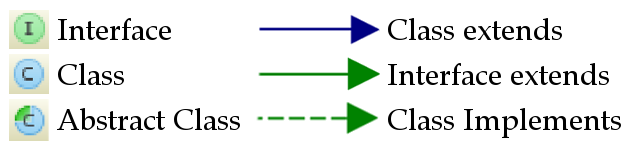
\includegraphics[width=\textwidth]{classDiagrams/classDiagramKey.png}
\caption{Key for the class diagrams in this report.}
\label{fig:classDiagramKey}
\end{figure}

\todo{Decide what to put here} Appendix \ref{sec:Generalising the Codebase Appendix} provides detailed coverage of both this change, and changes made to some of the other areas of the AIM codebase.

\section{Merge Schemes}
\label{sec:Merge Schemes}
\begin{tabular}{|c|c|c|}
\hline
Requirement Code & Acheived? \\
\hline
FS.81 & \cellcolor{red} \xmark \\
FS.91 & \cellcolor{red} \xmark \\
\hline
\end{tabular}
The original plan was to implement two merge schemes, an AIM based centralised protocol and a dentralised approach based on \citetitle{VanMiddlesworth2008} \citep{VanMiddlesworth2008}. However, implementation proved to be very difficult. 

The AIM protocol implementation was developed by examining the original AIM code and creating a modified version applicable to merges. Because the two systems are so similar, much of the code was duplicated. This could be refactored out a later date, but during development having full control over the actions taken by a vehicle without having to compromise to allow AIM to work correctly was very useful. In the end, despite this approach there were significant issues with the system. Despite using very similar approaches to AIM, almost identical in areas, vehicles would continue to arrive early to their reserved times and vehicles would also collide consistently at intersections.

The system also suffered from some more fundamental problems. Reservations for merges are only taken by the lead vehicle in each lane, as vehicles behind them shouldn't be able to reserve ahead of the lead vehicle. This leads to slow downs at the merge zone as secondary vehicles won't be able to make reservations until the lead vehicle has entered the merge. If secondary vehicles also have to compete with vehicles on the other lane then it is likely that at least one of them will have to stop at the merge. This is fine for four-way stops, but for a merge where maintaining vehicle flow is the primary aim, this system will be far less effective.

The AIM protocol also fails to ensure that one lane does not suffer for the benefit of the other. Reservations are granted on a first-come-first-serve basis (though this could be changed by implementing a different reservation policy) and this can lead to long periods of time where one lane fails to make reservations whilst the other passes vehicles through quickly. Again, this fails to maintain traffic flow, one of the key aims of a merging protocol.

- Queue
As a response to AIM, I developed an alternative centralised approach to the merge problem. Described in 

-- Response to AIM's failings
-- Describe how it was implemented

- Decentralised
-- Never implemented due to time constraints.

\section{Simulation}
\label{sec:Simulation}
\begin{tabular}{|c|c|c|}
\hline
Requirement Code & Acheived? \\
\hline
FS.12 & \cellcolor{green} \cmark \\
FS.13 & \cellcolor{green} \cmark \\
FS.22 & \cellcolor{green} \cmark \\
FS.32 & \cellcolor{green} \cmark \\
FS.42 & \cellcolor{green} \cmark \\
FS.71 & \cellcolor{green} \cmark \\
FS.73 & \cellcolor{green} \cmark \\
FS.172 & \cellcolor{red} \xmark \\
NS.3 & \cellcolor{green} \cmark \\
NS.4 & \cellcolor{green} \cmark \\
NS.8 & \cellcolor{green} \cmark \\
\hline
\end{tabular}

Each simulation consists of multiple interacting agents, which makes it a difficult problem to implement. Using some of the generalised AIM classes helped to reduce the amount of time it took to implement these components. However, using AIM did introduce some complications and parts of the code had to be rewritten to adjust for this.

\subsection{Drivers}
\label{subsec:Drivers}
Driver agents are responsible for manipulating the vehicles in the simulation. They make requests to centralised merge managers and act upon the responses they are given. Each driver acts as a finite state machine, performing specific sets of actions for each state. Vehicles and Drivers both extend from generalised Vehicle and Driver classes containing useful functions for following lanes, turning and determining distances. However, some of these methods proved to be flawed.

One of the main issues was the assumption that lanes and roads will always meet at 90\degree. This caused a number of small issues throughout development, but one key problem was turning. A turn through an intersection in the AIM simulator is done by forcing the vehicle to point to a coordinate further down the lane the vehicle is following. This point is always exactly the same distance away from the vehicle, such that when the vehicle reaches a corner, and the lane it's following changes, the vehicle will turn towards that point gradually. This distance proved too much for some merges, and resulted in the vehicle making turns too gradually. This was fixed by setting the turn distance to always be the distance from the point at which the vehicle enters the merge zone, to the merge zone exit. The target point would also always lie in the centre of the target lane. This caused merging vehicles to turn more tightly, freeing up the lane for more vehicles. Figure \ref{fig:turning} shows how these turns work.

\begin{figure}[htb]
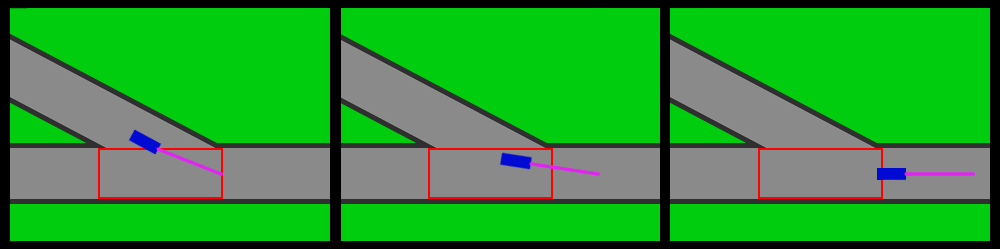
\includegraphics[width=\textwidth]{implementationDiagrams/turning.png}
\caption{Key for the class diagrams in this report.}
\label{fig:turning}
\end{figure}

Another problem came about due to collisions. AIM had provided a method called \emph{dontHitCarInFront} which calculates the distance from the vehicle to the vehicle in front and then takes action to avoid a collision, slowing down if necessary. This method turns out to not be completely effective. Even within the AIM simulations vehicles are colliding. Due to time constraints collision detection was removed from the project as I did not have time to go hunting for the error causing collisions. Overall it does not matter too much as the cars only collide momentarily before separating, but it does make it difficult to detect collision errors caused by merging algorithms. As far as I can tell, no collisions take place with the algorithm implemented, as it should be almost imposible, but without having a check in place this cannot be said for certain.

\subsection{Merge Managers}
\label{subsec:Merge Managers}
The role of a merge manager is to take requests from drivers and provide responses, controlling the flow of traffic through the merge zone. They were heavily influenced by the approaches taken by AIM. The AIM based merge manager replicated much of the intersection manager code introduced by AIM. At a later date this could be refactored to reduce duplication, but this would most likely also require changes to Driver and Vehicle, as each type of merge manager deals with different types of vehicles and drivers.

The final implementation of a merge manager, the QueueV2IManager, is designed similarly to AIM's V2IIntersectionManager, however much of the technical code is original and far simpler. This merge manager effectively just manages a queue and alerts vehicles when they are at the front of said queue. The AIM system is more complex, requiring the merge manager to monitor reservations and time the arrival of vehicles as they arrive. The AIM system relies very heavily on each vehicle arriving at their stated time and fails to handle vehicles well if they don't.

\subsection{Map}
\label{subsec:Map}
The simulation map stores all of the spawn points, lanes and merge managers for the simulation. The calcualtions for lane positions and spawn points were created using the designs in \ref{sec:Map}. 

By using some of the generalised components for calculating distances, creating the map was relatively straightforward, however, there were some components that failed to work as intended. The original AIM system assumes that every road meets at 90\degree and as such some methods were inappropriate for when lanes meet at other angles. One example of this is the no vehicle zone at the beginning of each lane. This zone stops multiple vehicles from spawning on top of each other. The original implementation calculated a Rectangle at the beginning of each lane, which works fine when lanes are at 90\degree. For my no vehicle zones, I had to draw a path around the start of each merge lane and create a shape from that. This more complicated approach was necessary due to the angles at which the merge lane can meet the target lane. 

The map also controls the spawn points creating the vehicles. Most spawning behaviours were based on the AIM spawn points. However, to enable consistent testing we wanted to be able to repeat the experiment with the same vehicles over and over again. To do this I created a new vehicle spawn type that uses a JSON file to spawn vehicles. The file contains a vehicle specification and a time. The spawner reads this data in and spawns a vehicle with the given specification at the indicated time. I also implemented this type of spawner into the AIM system. This means that comparisons between the performance of AIM and the Queue protocol are now possible.

\subsection{Simulation Control}
\label{subsec:Simulation Control}
The simulator itself is reponsible for triggering and monitoring the actions of each component of the simulation. It delivers messages between merge managers and vehicles and moves vehicles through the simulation according to their specified velocities and headings.

\section{Results Production}
\label{sec:Results Production}
\begin{tabular}{|c|c|c|}
\hline
Requirement Code & Acheived? \\
\hline
FS.62 & \cellcolor{green} \cmark \\
FS.63 & \cellcolor{green} \cmark \\
FS.64 & \cellcolor{green} \cmark \\
FS.65 & \cellcolor{green} \cmark \\
FS.66 & \cellcolor{red} \xmark \\
FS.67 & \cellcolor{red} \xmark \\
FS.68 & \cellcolor{green} \cmark \\
FS.69 & \cellcolor{red} \xmark \\
FS.6a & \cellcolor{red} \xmark \\
NS.7 & \cellcolor{green} \cmark \\
\hline
\end{tabular}
- Results generation to CSV file
- Drivers, spawners and simulations adapted to provide the relevant export information
- Setup in AIM as well
- Whay wasn't max accell stored?

\section{GUI}
\label{sec:GUI}
\begin{tabular}{|c|c|c|}
\hline
Requirement Code & Acheived? \\
\hline
FS.11 & \cellcolor{green} \cmark \\
FS.21 & \cellcolor{green} \cmark \\
FS.31 & \cellcolor{green} \cmark \\
FS.41 & \cellcolor{green} \cmark \\
FS.51 & \cellcolor{green} \cmark \\
FS.61 & \cellcolor{green} \cmark \\
FS.72 & \cellcolor{green} \cmark \\
FS.82 & \cellcolor{red} \xmark \\
FS.92 & \cellcolor{red} \xmark \\
FS.101 & \cellcolor{green} \cmark \\
FS.111 & \cellcolor{green} \cmark \\
FS.121 & \cellcolor{green} \cmark \\
FS.131 & \cellcolor{green} \cmark \\
FS.141 & \cellcolor{green} \cmark \\
FS.151 & \cellcolor{green} \cmark \\
FS.161 & \cellcolor{green} \cmark \\
FS.171 & \cellcolor{red} \xmark \\
NS.1 & \cellcolor{green} \cmark \\
NS.2 & \cellcolor{green} \cmark \\
NS.5 & \cellcolor{green} \cmark \\
NS.6 & \cellcolor{green} \cmark \\
\hline
\end{tabular}

The GUI for the project was built using Java Swing, extending the existing AIM GUI. New simulator types are given a separate tab in the application with their own simulator setup and a display screen. The display screen can be modified for each simulation type, showing the relevant information for that simulation. We moved away from the AIM full illustrated canvas implementation to a 'StatScreen' implementation which shows information in text format instead. The S2S simulations display the current simulation time, number of completed vehicles and throughput. They also display two tables, one containing information about the vehicles currently in the simulation, and another for vehicles that have left the simulation. Figure \ref{fig:s2sSimScreen} shows the simulation screen for S2S merges.

-- Consistent testing upload 

\begin{figure}[htb]
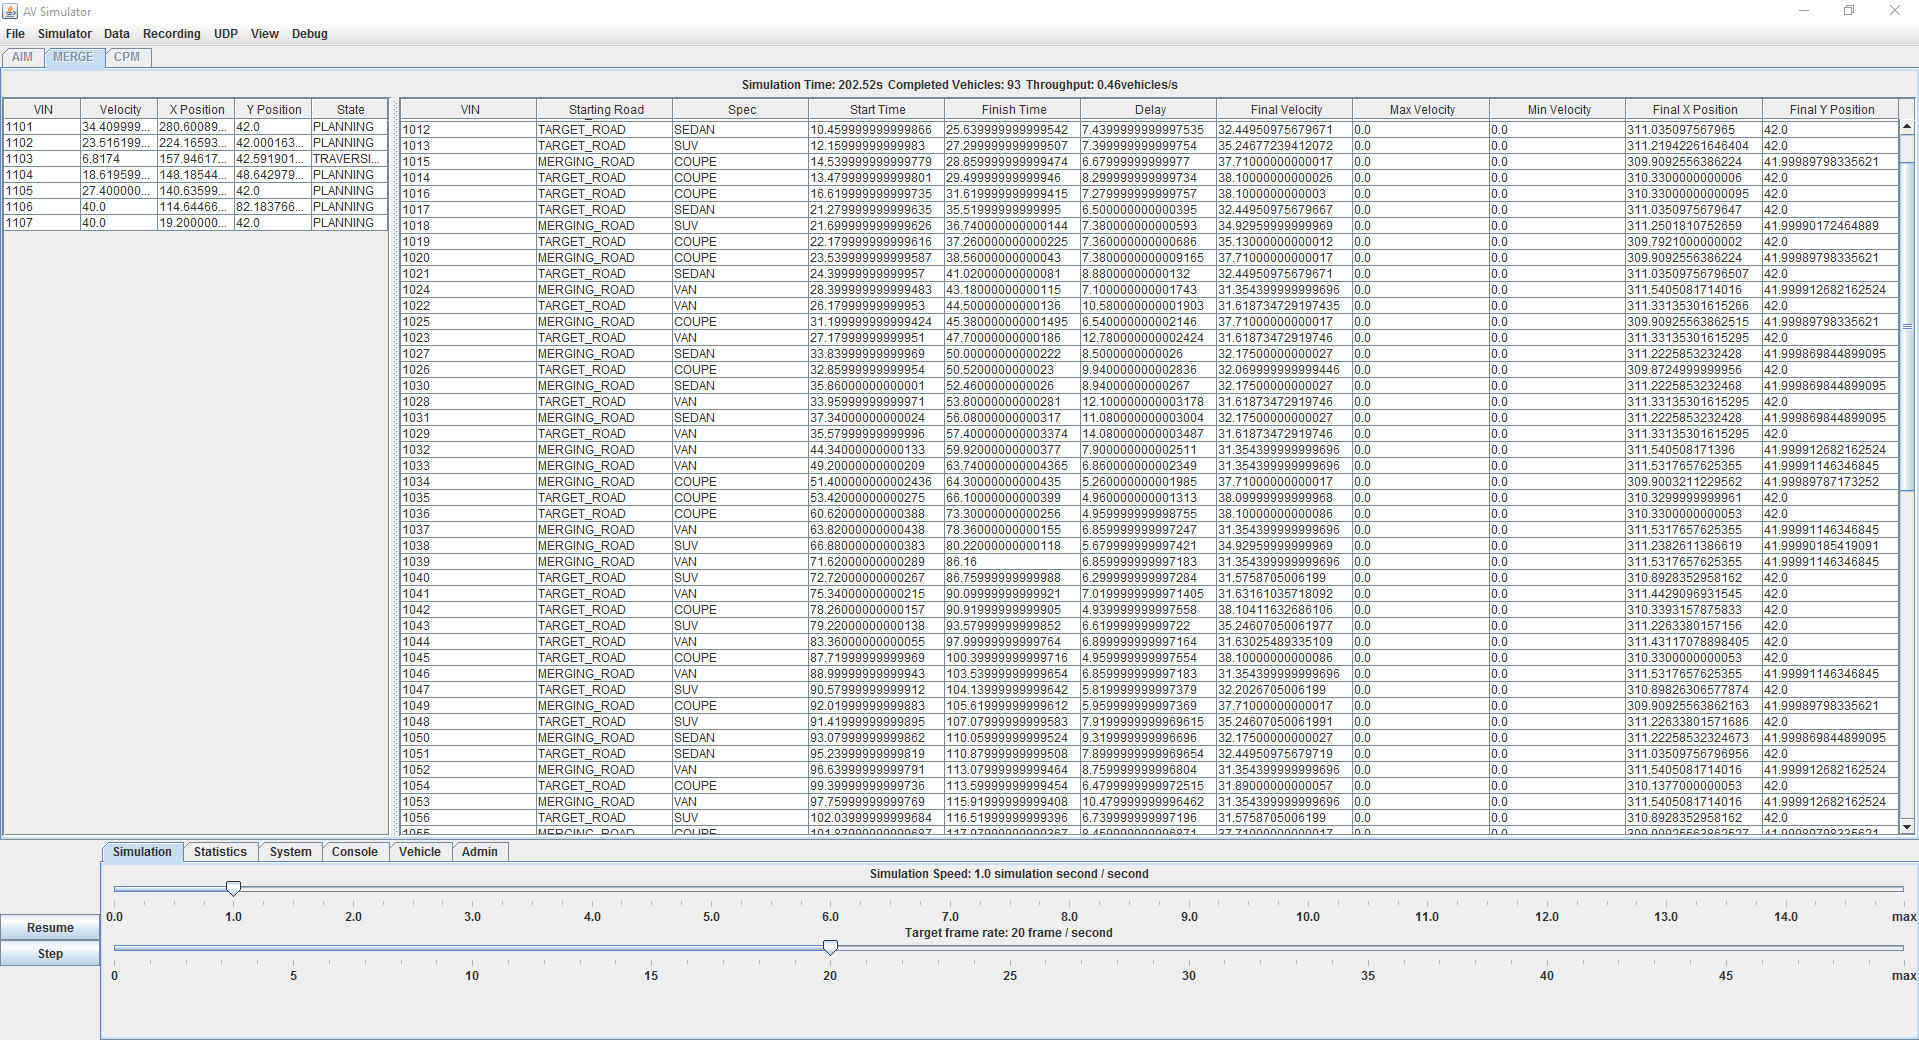
\includegraphics[width=\textwidth]{screenshots/s2sSimulationScreen.png}
\caption{The simulation screen for the S2S merge screen}
\label{fig:s2sSimScreen}
\end{figure}

Functional requirements \emph{FS.82} and \emph{FS.92} were not fully implemented as the AIM-like simulations and Decentralised simulations were never implemented in a fully working form. \emph{FS.171} was also never implemented due to the removal of collision detection from simulations. All other GUI requirements were completed.

\section{Maintainability and Testing}
\label{sec:Testing}
\begin{tabular}{|c|c|c|}
\hline
Requirement Code & Acheived? \\
\hline
NS.9 & \cellcolor{green} \cmark \\
NS.10 & \cellcolor{green} \cmark \\
\hline
\end{tabular}

\subsection{Unit Testing}
\label{subsec:Unit Testing}
Unit tests were mostly used to ensure getter and setter methods worked as expected. However, some unit tests were used to verify the behaviour of classes. To do this I used Mockito \citep{MockitoWebsite} to mock the behaviour of objects used by the test class so that I could prompt the test class into producing the expected results.

\subsection{Integration Tests}
\label{subsec:Integration Tests}


\chapter{Results}
\label{cha:Results}
The simulator was designed to allow for variance in merge angle, lead in distances, speed limits, and traffic levels. This means that we can experiment to see what effect each of these variables has on the effectiveness of the Queue protocol. We can also compare the Queue protocol to the AIM protocol, using the modified version of the AIM simulator described in \ref{sec:Merge Schemes}.

\section{Experimental Procedure}
\label{sec:Experimental Procedure}
All experiments were done using pre-generated spawn schedules. In each experiment I used 20 pairs of schedules (1 schedule per lane). Schedule pairs are identical for tests with the same speed limit and traffic density (or traffic rate). Vehicles spawned for 1000 simulated seconds, and all vehicles were allowed to complete. The spawn schedules would only fail to spawn a vehicle if the spawning area was occupied by another vehicle. This can cause reduced numbers of completed vehicles if the system becomes congested enough to cause queues up to the spawning area. 

\section{Comparing AIM and Queue Protocols}
\label{sec:Comparing AIM and Queue Protocols}
By using the modified AIM simulator described in \ref{sec:Merge Schemes} I obtained approximations for how well the AIM protocol handles merges.

The AIM simulator has a lead in and lead out distance for each lane of 150 metres and is limited to 90\degree merges. These settings were duplicated for the queue merge type. All of the lanes were set to have a speed limit of 20$\si{ms^{-1}}$ (44.7\si{mph} or 72\si{kph}). The traffic rate (vehicles/hour/lane (\si{vhl})) was altered to see how well the systems adjust to increasing levels of traffic.

In terms of reducing mean delay, both systems performed well at low traffic rates. From 500 to 1500\si{vhl} both systems kept mean delay below 2 seconds. AIM performed slightly better, hitting a mean delay 0.97\si{s} with a standard deviation of 1.35\si{s}, queue achieved a mean delay of 1.84\si{s} with a standard deviation of 2.22\si{s}. As the traffic rates increased however, the performance of the queue system degraded massively in comparison to AIM. At 2500\si{vhl} the queue system hit a mean delay of 45.78\si{s} with a standard deviation of 18.13\si{s}. In comparison, AIM hit a mean delay of 5.43\si{s} and a standard deviation of 6.25\si{s}. Even with a high standard deviation like this, it's clear that AIM outperforms the queue system in this respect. Figure \ref{fig:meanDelayTrafficRate} shows how the two systems compare.

\begin{figure}[htb]
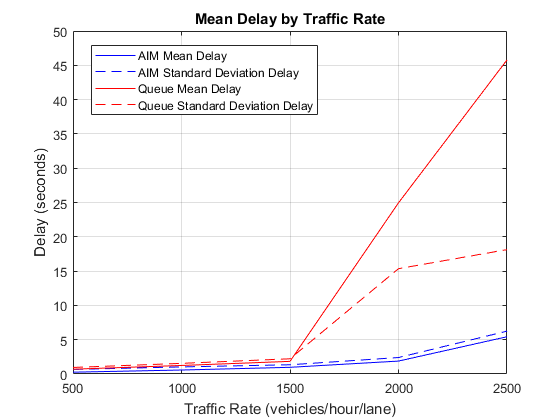
\includegraphics[width=\textwidth]{plots/trafficRate/meanDelay.png}
\caption{Plot showing mean delay/traffic rate performance by merge management system.}
\label{fig:meanDelayTrafficRate}
\end{figure}

In terms of balancing mean delay over both lanes, the queue system also fails to perform as well as AIM. At 500\si{vhl} the mean target lane delay for the queue system is 0.06\si{s}, with a standard deviation of 0.25\si{s}. For the merge lane, the delay is 1.36\si{s}, with a standard deviation of 0.95\si{s}. Comparatively AIM has a mean delay of 0.37\si{s}, with a standard deviation of 0.79\si{s}, for the target lane, and 0.16\si{s}, with a standard deviation of 0.47\si{s}, for the merge lane. 

At higher traffic rates the gap between the AIM lanes increases. At 2500\si{vhl} AIM has a mean delay of 1.75\si{s}, with a standard deviation of 1.54\si{s}, for the target lane, and 9.11\si{s}, with a standard deviation of 6.79\si{s}, for the merge lane. These times are still far better than the mean delays in the queue system. Figure \ref{fig:meanDelayByLaneTrafficRate} shows how each lane performs under each system.

\begin{figure}[htb]
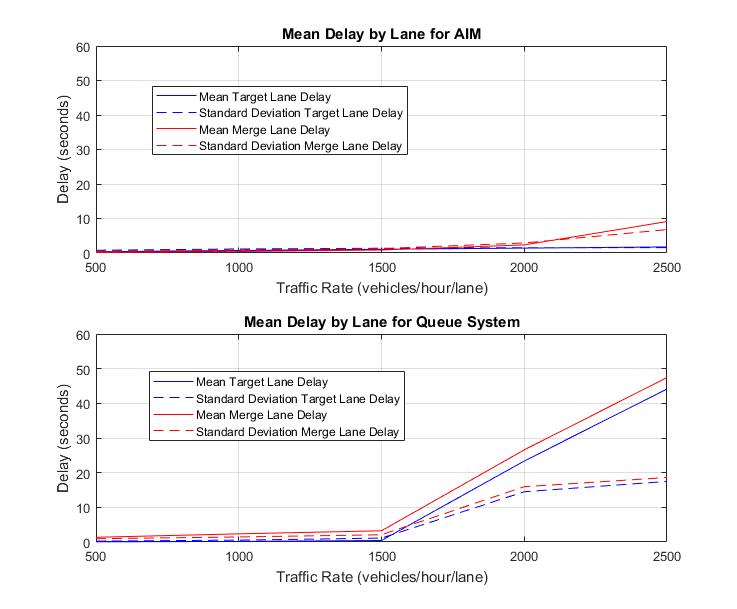
\includegraphics[width=\textwidth]{plots/trafficRate/meanDelayByLane.png}
\caption{Plots showing mean delay by lane for both merge management systems}
\label{fig:meanDelayByLaneTrafficRate}
\end{figure}

Both system manage to maintain similar throughputs until the traffic rate increases past 1500\si{vhl}. By 2500\si{vhl}, AIM can deal with an extra 366 vehicles per hour compared to the queue system. Figure \ref{fig:throughputTrafficRate} shows the throughputs for each system.

\begin{figure}[htb]
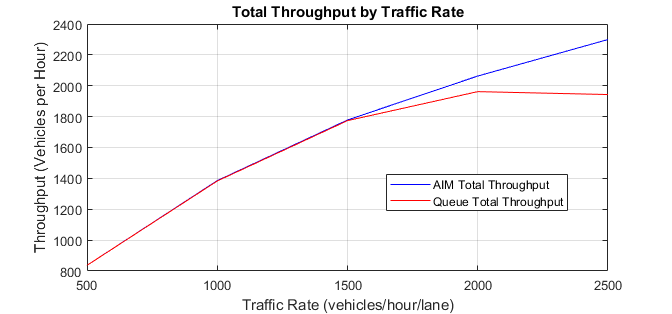
\includegraphics[width=\textwidth]{plots/trafficRate/throughput.png}
\caption{Plot showing throughput for both merge management systems}
\label{fig:throughputTrafficRate}
\end{figure}

These trends clearly demonstrate that AIM performs far more effectively at high traffic rates than the queue system. AIM makes better use of space-time, so when the roads begin getting more congested, this pays off in AIMs favour. The queue system ends up causing problems at these high traffic rates as it only allows one vehicle into the merge zone at any one time. A queue system would work well for controlling roads with lower traffic rates, however, if the roads are expected to deal with congestion or high volume fast flowing traffic, the AIM system becomes the only viable option of the two.

This test makes a good case for continuing attempts to develop an AIM based system for merges. This system would need to be able to work for other merge angles, as no research was conducted into the effectiveness of AIM at shallower angles. Further development would also need to done using a simulator which deals with some of the implementation problems found in the AIM simulator. As detailed in section \ref{sec:Implementation}, collisions and early arrival times were constant problems with attempts to implement an AIM-based merge system in the AIM simulator.

\section{The Effect of the Merge Angle}
\label{sec:The Effect of the Merge Angle}
The merge angle affects both the length of the merge zone and the angle at which vehicles join the target lane, affecting how far they're needed to turn. For the queue system to be effective, it should be able to deal with a range of merge angles.

For each test, the speed limit for both lanes was 20$\si{ms^{-1}}$ (44.7\si{mph} or 72\si{kph}) and each lane had a lead in distance of 150\si{m}. The traffic rate was set to 1000\si{vhl}.

At shallow angles the queue system performed very poorly. At the shallowest angle tested, 5\degree, the system had a mean delay of 138.98\si{s} with a standard deviation of 46.96\si{s}. After the merge angle increases to around 30\degree, performance has improved greatly with the mean delay reaching 13.12\si{s} with a standard deviation of 9.35\si{s}. By the time the merge zone has reached it's minimum length, the mean delay has decreased to 1.24\si{s} with a standard deviation of 1.55\si{s}. The delay is actually smaller at 85\degree at 1.23\si{s} but this is well with range of the standard deviation for 90\degree. The delay of both the target lane and merge lane follow very similar trends. Figure \ref{fig:meanDelayMergeAngle} shows how the delay decreases as the angle increases.

\begin{figure}[htb]
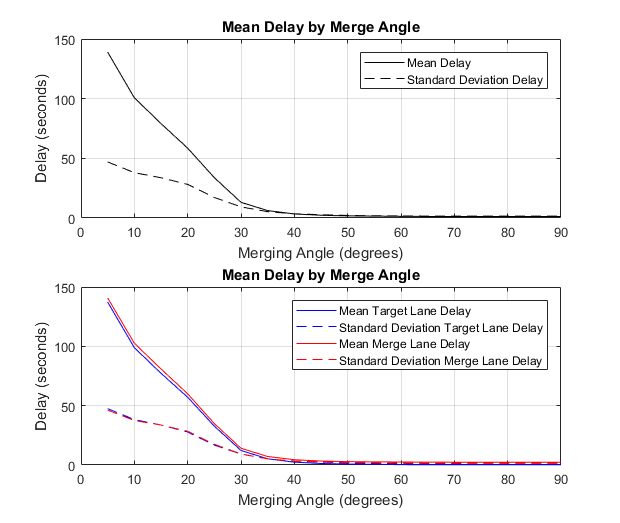
\includegraphics[width=\textwidth]{plots/mergeAngle/meanDelay.png}
\caption{Plot showing mean delay by merge angle}
\label{fig:meanDelayMergeAngle}
\end{figure}

In general throughput increases dramatically with the merge angle until around 35\degree where levels off dramatically. The data does show a dip in the merge lane throughput measurements from 40\degree to 60\degree. Investigation showed that this was an error with vehicle spawn system which dropped vehicles after detecting that there was still another vehicle in the spawn area. These were false detections due to the change in angle. A solution to the problem would have required separate spawn schedules for each angle which reduces the validity of the results. These results are considered to be outliers. Figure \ref{fig:throughputMergeAngle} shows how the throughput improves as the angle increases.

\begin{figure}[htb]
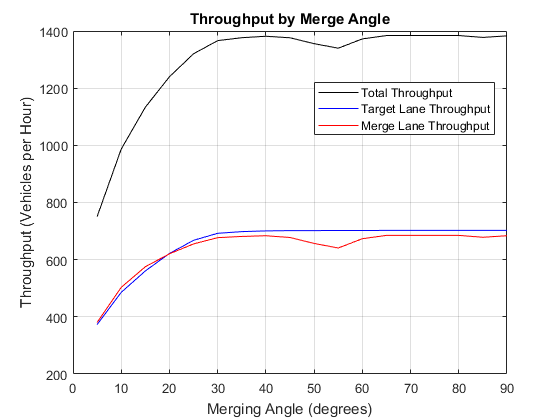
\includegraphics[width=\textwidth]{plots/mergeAngle/throughput.png}
\caption{Plot showing throughput by merge angle}
\label{fig:throughputMergeAngle}
\end{figure}

Shallow merge angles have such a drastic effect on performance because as the merge angle becomes shallower the merge zone gets longer. This means that the space time inefficiency of the queue system has a huge effect on performance as vehicles have to wait for longer before they can enter the merge. One approach for dealing with shallow merges is to introduce a slip road instead of a merge zone. This would require a different system, as queuing wouldn't be appropriate in that situation.

\section{The Effect of Lead in Distances}
\label{sec:The Effect of Lead in Distances}
The lead in distance adjustments affect how long vehicles have to organise and communicate with the queue system. Different lead in distance pairs were tested. The traffic rate was set to 1000\si{vhl}, the merge angle was 45\degree, and the speed limit was set to 20$\si{ms^{-1}}$ (44.7\si{mph} or 72\si{kph}).

Due to 150\si{m} distance limit on requests, lead ins at 100\si{m} were worse for the lane with the 100\si{m} lead in. The only exceptions were when both lanes had lead in distances of 100\si{m}.

If one lane has a 100\si{m} lead, then the other lane also suffers a performance hit. This affect is most noticeable when the target lane has the 100\si{m} lead, but this effect is also seen with the merge lane. Figure \ref{fig:meanDelayLeadIn} shows how the delay relates to the lead in distance.

\begin{figure}[htb]
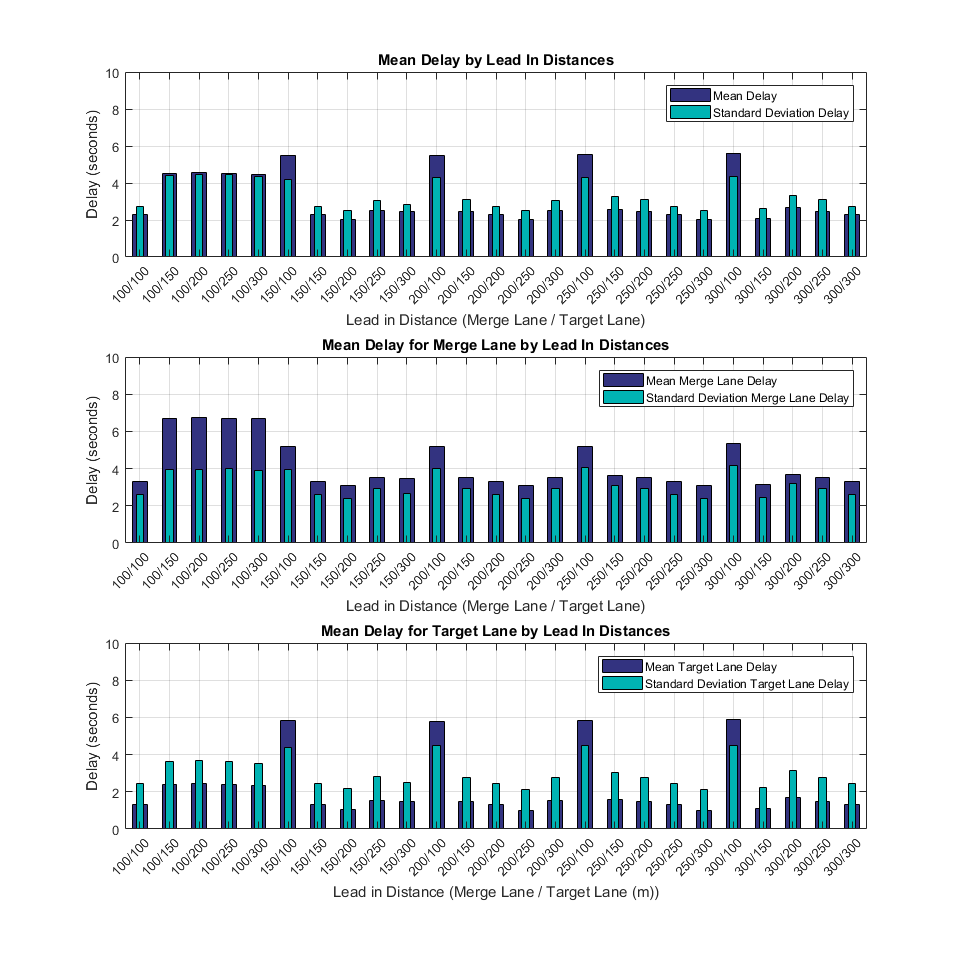
\includegraphics[width=\textwidth]{plots/leadIn/meanDelay.png}
\caption{Bar chart showing mean delay by lead in distance}
\label{fig:meanDelayLeadIn}
\end{figure}

Beyond 150\si{m} the lead in distance had very little effect on the performance of the system. Throughput remained relatively constant throughout.

\section{The Effect of Differing Speed Limits}
\label{sec:The Effect of Differing Speed Limits}
The speed limits of each lane and their difference impacts how well a vehicle can move into another lane and adjust to it's velocity. Many merges will be movements from lanes of differing speed, so its important that the queue system can handles these merges.

The traffic rate was set to 1000\si{vhl}, the merge angle was 45\degree, and the lead in distances were both set to 150\si{m}. Pairs of speeds were compared. The speed limits used were 10$\si{ms^{-1}}$, 20$\si{ms^{-1}}$, 30$\si{ms^{-1}}$, and 40$\si{ms^{-1}}$ (22.4\si{mph}, 44.7\si{mph}, 67.1\si{mph} and 89.5\si{mph} or 36\si{kph} 72\si{kph} 108\si{kph} and 144\si{kph} respectively). These speeds, excluding 40$\si{ms^{-1}}$, are very close to realistic speed limits and should provide insight into the real world applicability of the system.

The target lane suffers the most interference from the merge lane whenever the target lane's velocity is larger than the merge lane. This can be seen well in the relationship between a target lane speed limit of 30$\si{ms^{-1}}$ and a merge lane speed limit of 10$\si{ms^{-1}}$. The mean delay on the target lane is 13.92\si{s} with a standard deviation of 3.56\si{s}. Comparatively the merge lane had a mean delay of 4.01\si{s} with a standard deviation of 2.87\si{s}. 

Switching the lane speeds shows that the merge lane also experiences larger delays when the merge lane is travelling faster than the target lane. When the target lane has a speed limit of 10$\si{ms^{-1}}$ and the merge lane has a speed limit of 30$\si{ms^{-1}}$, the merge lane has a mean delay of 12.00\si{s} with a standard deviation of 3.00\si{s}. In this case the target lane has a mean delay of 0.34\si{s} with a standard deviation of 0.95\si{s}.

It should be noted that when the speed gaps are smaller the effect on the lanes is reduced. When the merge lane speed was 30$\si{ms^{-1}}$ and the target lane speed was 20$\si{ms^{-1}}$ the system performed about as well as when both lanes have a speed limit of 30$\si{ms^{-1}}$, at least on the target lane. It should also be noted that most of the speed limits containing a 40$\si{ms^{-1}}$ lane performed poorly. The velocity causes vehicles to accumulate too quickly for the queue system to be able to sort them out effectively. Figure \ref{fig:meanDelaySpeedLimit} shows how the mean delay is affected by difference speed limit pairs.

\begin{figure}[htb]
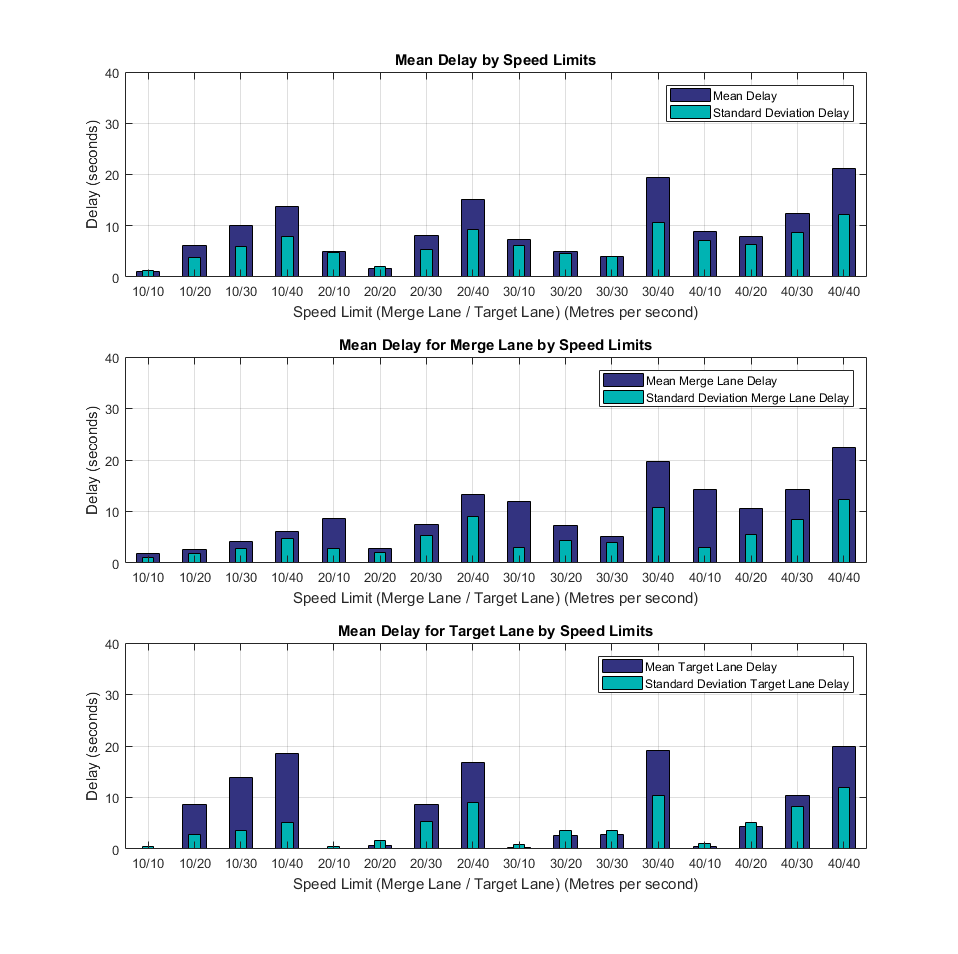
\includegraphics[width=\textwidth]{plots/speedLimit/meanDelay.png}
\caption{Bar chart showing mean delay by speed limit pair}
\label{fig:meanDelaySpeedLimit}
\end{figure}

The number of vehicles that complete for each lane is solely affected by the speed limit of the lane, the differences between the lanes has very little effect. The throughput is likewise only affected by the speed limits of each lane independently. Figure \ref{fig:throughputSpeedLimit} shows how the throughput is affected by the speed limits.

\begin{figure}[htb]
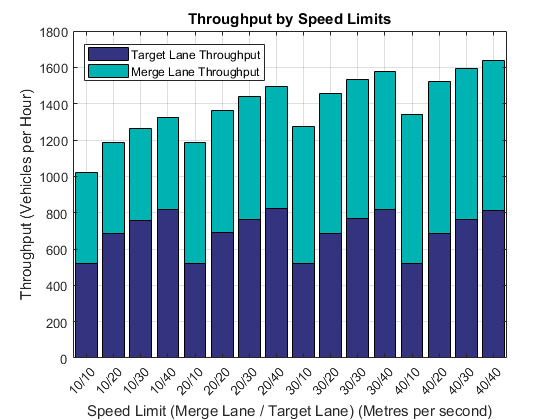
\includegraphics[width=\textwidth]{plots/speedLimit/throughput.png}
\caption{Bar chart showing throughput by speed limit pair}
\label{fig:throughputSpeedLimit}
\end{figure}

These results show that the queue system struggles to handle differences in velocity well, with the faster lane being impacted more heavily than the slower lane. This is because the faster lane is forced to slow down to accommodate the slower lane. In an ideal world a system should be able to slow down vehicles more gradually to allow vehicles in, before speeding up again. As it stands both the AIM and queue systems slow vehicles down at their maximum deceleration.




\bibliography{bibliography}

\end{document}